\documentclass[10pt,a4paper]{article}
\usepackage[utf8]{inputenc}
\usepackage[spanish]{babel}
\usepackage{amsmath, amsbsy, amssymb, amsthm, amsfonts}
\usepackage{graphicx}
\usepackage{multicol}
\usepackage{titling}
\usepackage{titlesec}
\usepackage{array}
\usepackage{bm}
\usepackage{afterpage}
\usepackage{float}
\usepackage{epstopdf}
\usepackage{longtable}
\usepackage{xcolor}
\usepackage{epigraph} 
\setlength\epigraphwidth{1.5\textwidth}
\usepackage{subfigure}
\usepackage{anyfontsize}
\usepackage{listings}
\renewcommand{\lstlistingname}{Programa}% Listing -> Programa
\renewcommand{\lstlistlistingname}{List of \lstlistingname s}
\usepackage[left=2cm,right=2cm,top=2cm,bottom=2cm]{geometry}
\usepackage[colorlinks=true,
            linkcolor=blue,
            citecolor=blue,
            urlcolor=blue]{hyperref}
 %%%%%%%%%%%%%%%%%%%%%%%%%%%%%%%%%%%%%%%%%%%%%%%%%%%%%%%%%%%%%%%%%%%%%%%%%%%%%%%% 
%%% ~ Arduino Language - Arduino IDE Colors ~                                  %%%
%%%                                                                            %%%
%%% Kyle Rocha-Brownell | 10/2/2017 | No Licence                               %%%
%%% -------------------------------------------------------------------------- %%%
%%%                                                                            %%%
%%% Place this file in your working directory (next to the latex file you're   %%%
%%% working on).  To add it to your project, place:                            %%%
%%%     %%%%%%%%%%%%%%%%%%%%%%%%%%%%%%%%%%%%%%%%%%%%%%%%%%%%%%%%%%%%%%%%%%%%%%%%%%%%%%%% 
%%% ~ Arduino Language - Arduino IDE Colors ~                                  %%%
%%%                                                                            %%%
%%% Kyle Rocha-Brownell | 10/2/2017 | No Licence                               %%%
%%% -------------------------------------------------------------------------- %%%
%%%                                                                            %%%
%%% Place this file in your working directory (next to the latex file you're   %%%
%%% working on).  To add it to your project, place:                            %%%
%%%     %%%%%%%%%%%%%%%%%%%%%%%%%%%%%%%%%%%%%%%%%%%%%%%%%%%%%%%%%%%%%%%%%%%%%%%%%%%%%%%% 
%%% ~ Arduino Language - Arduino IDE Colors ~                                  %%%
%%%                                                                            %%%
%%% Kyle Rocha-Brownell | 10/2/2017 | No Licence                               %%%
%%% -------------------------------------------------------------------------- %%%
%%%                                                                            %%%
%%% Place this file in your working directory (next to the latex file you're   %%%
%%% working on).  To add it to your project, place:                            %%%
%%%    \input{arduinoLanguage.tex}                                             %%%
%%% somewhere before \begin{document} in your latex file.                      %%%
%%%                                                                            %%%
%%% In your document, place your arduino code between:                         %%%
%%%   \begin{lstlisting}[language=Arduino]                                     %%%
%%% and:                                                                       %%%
%%%   \end{lstlisting}                                                         %%%
%%%                                                                            %%%
%%% Or create your own style to add non-built-in functions and variables.      %%%
%%%                                                                            %%%
 %%%%%%%%%%%%%%%%%%%%%%%%%%%%%%%%%%%%%%%%%%%%%%%%%%%%%%%%%%%%%%%%%%%%%%%%%%%%%%%% 

\usepackage{color}
\usepackage{listings}    
\usepackage{courier}

%%% Define Custom IDE Colors %%%
\definecolor{arduinoGreen}    {rgb} {0.17, 0.43, 0.01}
\definecolor{arduinoGrey}     {rgb} {0.47, 0.47, 0.33}
\definecolor{arduinoOrange}   {rgb} {0.8 , 0.4 , 0   }
\definecolor{arduinoBlue}     {rgb} {0.01, 0.61, 0.98}
\definecolor{arduinoDarkBlue} {rgb} {0.0 , 0.2 , 0.5 }

%%% Define Arduino Language %%%
\lstdefinelanguage{Arduino}{
  language=C++, % begin with default C++ settings 
%
%
  %%% Keyword Color Group 1 %%%  (called KEYWORD3 by arduino)
  keywordstyle=\color{arduinoGreen},   
  deletekeywords={  % remove all arduino keywords that might be in c++
                break, case, override, final, continue, default, do, else, for, 
                if, return, goto, switch, throw, try, while, setup, loop, export, 
                not, or, and, xor, include, define, elif, else, error, if, ifdef, 
                ifndef, pragma, warning,
                HIGH, LOW, INPUT, INPUT_PULLUP, OUTPUT, DEC, BIN, HEX, OCT, PI, 
                HALF_PI, TWO_PI, LSBFIRST, MSBFIRST, CHANGE, FALLING, RISING, 
                DEFAULT, EXTERNAL, INTERNAL, INTERNAL1V1, INTERNAL2V56, LED_BUILTIN, 
                LED_BUILTIN_RX, LED_BUILTIN_TX, DIGITAL_MESSAGE, FIRMATA_STRING, 
                ANALOG_MESSAGE, REPORT_DIGITAL, REPORT_ANALOG, SET_PIN_MODE, 
                SYSTEM_RESET, SYSEX_START, auto, int8_t, int16_t, int32_t, int64_t, 
                uint8_t, uint16_t, uint32_t, uint64_t, char16_t, char32_t, operator, 
                enum, delete, bool, boolean, byte, char, const, false, float, double, 
                null, NULL, int, long, new, private, protected, public, short, 
                signed, static, volatile, String, void, true, unsigned, word, array, 
                sizeof, dynamic_cast, typedef, const_cast, struct, static_cast, union, 
                friend, extern, class, reinterpret_cast, register, explicit, inline, 
                _Bool, complex, _Complex, _Imaginary, atomic_bool, atomic_char, 
                atomic_schar, atomic_uchar, atomic_short, atomic_ushort, atomic_int, 
                atomic_uint, atomic_long, atomic_ulong, atomic_llong, atomic_ullong, 
                virtual, PROGMEM,
                Serial, Serial1, Serial2, Serial3, SerialUSB, Keyboard, Mouse,
                abs, acos, asin, atan, atan2, ceil, constrain, cos, degrees, exp, 
                floor, log, map, max, min, radians, random, randomSeed, round, sin, 
                sq, sqrt, tan, pow, bitRead, bitWrite, bitSet, bitClear, bit, 
                highByte, lowByte, analogReference, analogRead, 
                analogReadResolution, analogWrite, analogWriteResolution, 
                attachInterrupt, detachInterrupt, digitalPinToInterrupt, delay, 
                delayMicroseconds, digitalWrite, digitalRead, interrupts, millis, 
                micros, noInterrupts, noTone, pinMode, pulseIn, pulseInLong, shiftIn, 
                shiftOut, tone, yield, Stream, begin, end, peek, read, print, 
                println, available, availableForWrite, flush, setTimeout, find, 
                findUntil, parseInt, parseFloat, readBytes, readBytesUntil, readString, 
                readStringUntil, trim, toUpperCase, toLowerCase, charAt, compareTo, 
                concat, endsWith, startsWith, equals, equalsIgnoreCase, getBytes, 
                indexOf, lastIndexOf, length, replace, setCharAt, substring, 
                toCharArray, toInt, press, release, releaseAll, accept, click, move, 
                isPressed, isAlphaNumeric, isAlpha, isAscii, isWhitespace, isControl, 
                isDigit, isGraph, isLowerCase, isPrintable, isPunct, isSpace, 
                isUpperCase, isHexadecimalDigit, 
                }, 
  morekeywords={   % add arduino structures to group 1
                break, case, override, final, continue, default, do, else, for, 
                if, return, goto, switch, throw, try, while, setup, loop, export, 
                not, or, and, xor, include, define, elif, else, error, if, ifdef, 
                ifndef, pragma, warning,
                }, 
% 
%
  %%% Keyword Color Group 2 %%%  (called LITERAL1 by arduino)
  keywordstyle=[2]\color{arduinoBlue},   
  keywords=[2]{   % add variables and dataTypes as 2nd group  
                HIGH, LOW, INPUT, INPUT_PULLUP, OUTPUT, DEC, BIN, HEX, OCT, PI, 
                HALF_PI, TWO_PI, LSBFIRST, MSBFIRST, CHANGE, FALLING, RISING, 
                DEFAULT, EXTERNAL, INTERNAL, INTERNAL1V1, INTERNAL2V56, LED_BUILTIN, 
                LED_BUILTIN_RX, LED_BUILTIN_TX, DIGITAL_MESSAGE, FIRMATA_STRING, 
                ANALOG_MESSAGE, REPORT_DIGITAL, REPORT_ANALOG, SET_PIN_MODE, 
                SYSTEM_RESET, SYSEX_START, auto, int8_t, int16_t, int32_t, int64_t, 
                uint8_t, uint16_t, uint32_t, uint64_t, char16_t, char32_t, operator, 
                enum, delete, bool, boolean, byte, char, const, false, float, double, 
                null, NULL, int, long, new, private, protected, public, short, 
                signed, static, volatile, String, void, true, unsigned, word, array, 
                sizeof, dynamic_cast, typedef, const_cast, struct, static_cast, union, 
                friend, extern, class, reinterpret_cast, register, explicit, inline, 
                _Bool, complex, _Complex, _Imaginary, atomic_bool, atomic_char, 
                atomic_schar, atomic_uchar, atomic_short, atomic_ushort, atomic_int, 
                atomic_uint, atomic_long, atomic_ulong, atomic_llong, atomic_ullong, 
                virtual, PROGMEM,
                },  
% 
%
  %%% Keyword Color Group 3 %%%  (called KEYWORD1 by arduino)
  keywordstyle=[3]\bfseries\color{arduinoOrange},
  keywords=[3]{  % add built-in functions as a 3rd group
                Serial, Serial1, Serial2, Serial3, SerialUSB, Keyboard, Mouse, EEPROM,
                TimerOne},      
%
%
  %%% Keyword Color Group 4 %%%  (called KEYWORD2 by arduino)
  keywordstyle=[4]\color{arduinoOrange},
  keywords=[4]{  % add more built-in functions as a 4th group
                abs, acos, asin, atan, atan2, ceil, constrain, cos, degrees, exp, 
                floor, log, map, max, min, radians, random, randomSeed, round, sin, 
                sq, sqrt, tan, pow, bitRead, bitWrite, bitSet, bitClear, bit, 
                highByte, lowByte, analogReference, analogRead, 
                analogReadResolution, analogWrite, analogWriteResolution, 
                attachInterrupt, detachInterrupt, digitalPinToInterrupt, delay, 
                delayMicroseconds, digitalWrite, digitalRead, interrupts, millis, 
                micros, noInterrupts, noTone, pinMode, pulseIn, pulseInLong, shiftIn, 
                shiftOut, tone, yield, Stream, begin, end, peek, read, print, 
                println, available, availableForWrite, flush, setTimeout, find, 
                findUntil, parseInt, parseFloat, readBytes, readBytesUntil, readString, 
                readStringUntil, trim, toUpperCase, toLowerCase, charAt, compareTo, 
                concat, endsWith, startsWith, equals, equalsIgnoreCase, getBytes, 
                indexOf, lastIndexOf, length, replace, setCharAt, substring, 
                toCharArray, toInt, press, release, releaseAll, accept, click, move, 
                isPressed, isAlphaNumeric, isAlpha, isAscii, isWhitespace, isControl, 
                isDigit, isGraph, isLowerCase, isPrintable, isPunct, isSpace, 
                isUpperCase, isHexadecimalDigit, 
                },      
%
%
  %%% Set Other Colors %%%
  stringstyle=\color{arduinoDarkBlue},    
  commentstyle=\color{arduinoGrey},    
%          
%   
  %%%% Line Numbering %%%%
   numbers=left,                    
  numbersep=5pt,                   
  numberstyle=\color{arduinoGrey},    
  %stepnumber=2,                      % show every 2 line numbers
%
%
  %%%% Code Box Style %%%%
  breaklines=true,                    % wordwrapping
  tabsize=2,
  frame=shadowbox,
  rulesepcolor=\color{arduinoBlue},         
  basicstyle=\ttfamily  
}                                             %%%
%%% somewhere before \begin{document} in your latex file.                      %%%
%%%                                                                            %%%
%%% In your document, place your arduino code between:                         %%%
%%%   \begin{lstlisting}[language=Arduino]                                     %%%
%%% and:                                                                       %%%
%%%   \end{lstlisting}                                                         %%%
%%%                                                                            %%%
%%% Or create your own style to add non-built-in functions and variables.      %%%
%%%                                                                            %%%
 %%%%%%%%%%%%%%%%%%%%%%%%%%%%%%%%%%%%%%%%%%%%%%%%%%%%%%%%%%%%%%%%%%%%%%%%%%%%%%%% 

\usepackage{color}
\usepackage{listings}    
\usepackage{courier}

%%% Define Custom IDE Colors %%%
\definecolor{arduinoGreen}    {rgb} {0.17, 0.43, 0.01}
\definecolor{arduinoGrey}     {rgb} {0.47, 0.47, 0.33}
\definecolor{arduinoOrange}   {rgb} {0.8 , 0.4 , 0   }
\definecolor{arduinoBlue}     {rgb} {0.01, 0.61, 0.98}
\definecolor{arduinoDarkBlue} {rgb} {0.0 , 0.2 , 0.5 }

%%% Define Arduino Language %%%
\lstdefinelanguage{Arduino}{
  language=C++, % begin with default C++ settings 
%
%
  %%% Keyword Color Group 1 %%%  (called KEYWORD3 by arduino)
  keywordstyle=\color{arduinoGreen},   
  deletekeywords={  % remove all arduino keywords that might be in c++
                break, case, override, final, continue, default, do, else, for, 
                if, return, goto, switch, throw, try, while, setup, loop, export, 
                not, or, and, xor, include, define, elif, else, error, if, ifdef, 
                ifndef, pragma, warning,
                HIGH, LOW, INPUT, INPUT_PULLUP, OUTPUT, DEC, BIN, HEX, OCT, PI, 
                HALF_PI, TWO_PI, LSBFIRST, MSBFIRST, CHANGE, FALLING, RISING, 
                DEFAULT, EXTERNAL, INTERNAL, INTERNAL1V1, INTERNAL2V56, LED_BUILTIN, 
                LED_BUILTIN_RX, LED_BUILTIN_TX, DIGITAL_MESSAGE, FIRMATA_STRING, 
                ANALOG_MESSAGE, REPORT_DIGITAL, REPORT_ANALOG, SET_PIN_MODE, 
                SYSTEM_RESET, SYSEX_START, auto, int8_t, int16_t, int32_t, int64_t, 
                uint8_t, uint16_t, uint32_t, uint64_t, char16_t, char32_t, operator, 
                enum, delete, bool, boolean, byte, char, const, false, float, double, 
                null, NULL, int, long, new, private, protected, public, short, 
                signed, static, volatile, String, void, true, unsigned, word, array, 
                sizeof, dynamic_cast, typedef, const_cast, struct, static_cast, union, 
                friend, extern, class, reinterpret_cast, register, explicit, inline, 
                _Bool, complex, _Complex, _Imaginary, atomic_bool, atomic_char, 
                atomic_schar, atomic_uchar, atomic_short, atomic_ushort, atomic_int, 
                atomic_uint, atomic_long, atomic_ulong, atomic_llong, atomic_ullong, 
                virtual, PROGMEM,
                Serial, Serial1, Serial2, Serial3, SerialUSB, Keyboard, Mouse,
                abs, acos, asin, atan, atan2, ceil, constrain, cos, degrees, exp, 
                floor, log, map, max, min, radians, random, randomSeed, round, sin, 
                sq, sqrt, tan, pow, bitRead, bitWrite, bitSet, bitClear, bit, 
                highByte, lowByte, analogReference, analogRead, 
                analogReadResolution, analogWrite, analogWriteResolution, 
                attachInterrupt, detachInterrupt, digitalPinToInterrupt, delay, 
                delayMicroseconds, digitalWrite, digitalRead, interrupts, millis, 
                micros, noInterrupts, noTone, pinMode, pulseIn, pulseInLong, shiftIn, 
                shiftOut, tone, yield, Stream, begin, end, peek, read, print, 
                println, available, availableForWrite, flush, setTimeout, find, 
                findUntil, parseInt, parseFloat, readBytes, readBytesUntil, readString, 
                readStringUntil, trim, toUpperCase, toLowerCase, charAt, compareTo, 
                concat, endsWith, startsWith, equals, equalsIgnoreCase, getBytes, 
                indexOf, lastIndexOf, length, replace, setCharAt, substring, 
                toCharArray, toInt, press, release, releaseAll, accept, click, move, 
                isPressed, isAlphaNumeric, isAlpha, isAscii, isWhitespace, isControl, 
                isDigit, isGraph, isLowerCase, isPrintable, isPunct, isSpace, 
                isUpperCase, isHexadecimalDigit, 
                }, 
  morekeywords={   % add arduino structures to group 1
                break, case, override, final, continue, default, do, else, for, 
                if, return, goto, switch, throw, try, while, setup, loop, export, 
                not, or, and, xor, include, define, elif, else, error, if, ifdef, 
                ifndef, pragma, warning,
                }, 
% 
%
  %%% Keyword Color Group 2 %%%  (called LITERAL1 by arduino)
  keywordstyle=[2]\color{arduinoBlue},   
  keywords=[2]{   % add variables and dataTypes as 2nd group  
                HIGH, LOW, INPUT, INPUT_PULLUP, OUTPUT, DEC, BIN, HEX, OCT, PI, 
                HALF_PI, TWO_PI, LSBFIRST, MSBFIRST, CHANGE, FALLING, RISING, 
                DEFAULT, EXTERNAL, INTERNAL, INTERNAL1V1, INTERNAL2V56, LED_BUILTIN, 
                LED_BUILTIN_RX, LED_BUILTIN_TX, DIGITAL_MESSAGE, FIRMATA_STRING, 
                ANALOG_MESSAGE, REPORT_DIGITAL, REPORT_ANALOG, SET_PIN_MODE, 
                SYSTEM_RESET, SYSEX_START, auto, int8_t, int16_t, int32_t, int64_t, 
                uint8_t, uint16_t, uint32_t, uint64_t, char16_t, char32_t, operator, 
                enum, delete, bool, boolean, byte, char, const, false, float, double, 
                null, NULL, int, long, new, private, protected, public, short, 
                signed, static, volatile, String, void, true, unsigned, word, array, 
                sizeof, dynamic_cast, typedef, const_cast, struct, static_cast, union, 
                friend, extern, class, reinterpret_cast, register, explicit, inline, 
                _Bool, complex, _Complex, _Imaginary, atomic_bool, atomic_char, 
                atomic_schar, atomic_uchar, atomic_short, atomic_ushort, atomic_int, 
                atomic_uint, atomic_long, atomic_ulong, atomic_llong, atomic_ullong, 
                virtual, PROGMEM,
                },  
% 
%
  %%% Keyword Color Group 3 %%%  (called KEYWORD1 by arduino)
  keywordstyle=[3]\bfseries\color{arduinoOrange},
  keywords=[3]{  % add built-in functions as a 3rd group
                Serial, Serial1, Serial2, Serial3, SerialUSB, Keyboard, Mouse, EEPROM,
                TimerOne},      
%
%
  %%% Keyword Color Group 4 %%%  (called KEYWORD2 by arduino)
  keywordstyle=[4]\color{arduinoOrange},
  keywords=[4]{  % add more built-in functions as a 4th group
                abs, acos, asin, atan, atan2, ceil, constrain, cos, degrees, exp, 
                floor, log, map, max, min, radians, random, randomSeed, round, sin, 
                sq, sqrt, tan, pow, bitRead, bitWrite, bitSet, bitClear, bit, 
                highByte, lowByte, analogReference, analogRead, 
                analogReadResolution, analogWrite, analogWriteResolution, 
                attachInterrupt, detachInterrupt, digitalPinToInterrupt, delay, 
                delayMicroseconds, digitalWrite, digitalRead, interrupts, millis, 
                micros, noInterrupts, noTone, pinMode, pulseIn, pulseInLong, shiftIn, 
                shiftOut, tone, yield, Stream, begin, end, peek, read, print, 
                println, available, availableForWrite, flush, setTimeout, find, 
                findUntil, parseInt, parseFloat, readBytes, readBytesUntil, readString, 
                readStringUntil, trim, toUpperCase, toLowerCase, charAt, compareTo, 
                concat, endsWith, startsWith, equals, equalsIgnoreCase, getBytes, 
                indexOf, lastIndexOf, length, replace, setCharAt, substring, 
                toCharArray, toInt, press, release, releaseAll, accept, click, move, 
                isPressed, isAlphaNumeric, isAlpha, isAscii, isWhitespace, isControl, 
                isDigit, isGraph, isLowerCase, isPrintable, isPunct, isSpace, 
                isUpperCase, isHexadecimalDigit, 
                },      
%
%
  %%% Set Other Colors %%%
  stringstyle=\color{arduinoDarkBlue},    
  commentstyle=\color{arduinoGrey},    
%          
%   
  %%%% Line Numbering %%%%
   numbers=left,                    
  numbersep=5pt,                   
  numberstyle=\color{arduinoGrey},    
  %stepnumber=2,                      % show every 2 line numbers
%
%
  %%%% Code Box Style %%%%
  breaklines=true,                    % wordwrapping
  tabsize=2,
  frame=shadowbox,
  rulesepcolor=\color{arduinoBlue},         
  basicstyle=\ttfamily  
}                                             %%%
%%% somewhere before \begin{document} in your latex file.                      %%%
%%%                                                                            %%%
%%% In your document, place your arduino code between:                         %%%
%%%   \begin{lstlisting}[language=Arduino]                                     %%%
%%% and:                                                                       %%%
%%%   \end{lstlisting}                                                         %%%
%%%                                                                            %%%
%%% Or create your own style to add non-built-in functions and variables.      %%%
%%%                                                                            %%%
 %%%%%%%%%%%%%%%%%%%%%%%%%%%%%%%%%%%%%%%%%%%%%%%%%%%%%%%%%%%%%%%%%%%%%%%%%%%%%%%% 

\usepackage{color}
\usepackage{listings}    
\usepackage{courier}

%%% Define Custom IDE Colors %%%
\definecolor{arduinoGreen}    {rgb} {0.17, 0.43, 0.01}
\definecolor{arduinoGrey}     {rgb} {0.47, 0.47, 0.33}
\definecolor{arduinoOrange}   {rgb} {0.8 , 0.4 , 0   }
\definecolor{arduinoBlue}     {rgb} {0.01, 0.61, 0.98}
\definecolor{arduinoDarkBlue} {rgb} {0.0 , 0.2 , 0.5 }

%%% Define Arduino Language %%%
\lstdefinelanguage{Arduino}{
  language=C++, % begin with default C++ settings 
%
%
  %%% Keyword Color Group 1 %%%  (called KEYWORD3 by arduino)
  keywordstyle=\color{arduinoGreen},   
  deletekeywords={  % remove all arduino keywords that might be in c++
                break, case, override, final, continue, default, do, else, for, 
                if, return, goto, switch, throw, try, while, setup, loop, export, 
                not, or, and, xor, include, define, elif, else, error, if, ifdef, 
                ifndef, pragma, warning,
                HIGH, LOW, INPUT, INPUT_PULLUP, OUTPUT, DEC, BIN, HEX, OCT, PI, 
                HALF_PI, TWO_PI, LSBFIRST, MSBFIRST, CHANGE, FALLING, RISING, 
                DEFAULT, EXTERNAL, INTERNAL, INTERNAL1V1, INTERNAL2V56, LED_BUILTIN, 
                LED_BUILTIN_RX, LED_BUILTIN_TX, DIGITAL_MESSAGE, FIRMATA_STRING, 
                ANALOG_MESSAGE, REPORT_DIGITAL, REPORT_ANALOG, SET_PIN_MODE, 
                SYSTEM_RESET, SYSEX_START, auto, int8_t, int16_t, int32_t, int64_t, 
                uint8_t, uint16_t, uint32_t, uint64_t, char16_t, char32_t, operator, 
                enum, delete, bool, boolean, byte, char, const, false, float, double, 
                null, NULL, int, long, new, private, protected, public, short, 
                signed, static, volatile, String, void, true, unsigned, word, array, 
                sizeof, dynamic_cast, typedef, const_cast, struct, static_cast, union, 
                friend, extern, class, reinterpret_cast, register, explicit, inline, 
                _Bool, complex, _Complex, _Imaginary, atomic_bool, atomic_char, 
                atomic_schar, atomic_uchar, atomic_short, atomic_ushort, atomic_int, 
                atomic_uint, atomic_long, atomic_ulong, atomic_llong, atomic_ullong, 
                virtual, PROGMEM,
                Serial, Serial1, Serial2, Serial3, SerialUSB, Keyboard, Mouse,
                abs, acos, asin, atan, atan2, ceil, constrain, cos, degrees, exp, 
                floor, log, map, max, min, radians, random, randomSeed, round, sin, 
                sq, sqrt, tan, pow, bitRead, bitWrite, bitSet, bitClear, bit, 
                highByte, lowByte, analogReference, analogRead, 
                analogReadResolution, analogWrite, analogWriteResolution, 
                attachInterrupt, detachInterrupt, digitalPinToInterrupt, delay, 
                delayMicroseconds, digitalWrite, digitalRead, interrupts, millis, 
                micros, noInterrupts, noTone, pinMode, pulseIn, pulseInLong, shiftIn, 
                shiftOut, tone, yield, Stream, begin, end, peek, read, print, 
                println, available, availableForWrite, flush, setTimeout, find, 
                findUntil, parseInt, parseFloat, readBytes, readBytesUntil, readString, 
                readStringUntil, trim, toUpperCase, toLowerCase, charAt, compareTo, 
                concat, endsWith, startsWith, equals, equalsIgnoreCase, getBytes, 
                indexOf, lastIndexOf, length, replace, setCharAt, substring, 
                toCharArray, toInt, press, release, releaseAll, accept, click, move, 
                isPressed, isAlphaNumeric, isAlpha, isAscii, isWhitespace, isControl, 
                isDigit, isGraph, isLowerCase, isPrintable, isPunct, isSpace, 
                isUpperCase, isHexadecimalDigit, 
                }, 
  morekeywords={   % add arduino structures to group 1
                break, case, override, final, continue, default, do, else, for, 
                if, return, goto, switch, throw, try, while, setup, loop, export, 
                not, or, and, xor, include, define, elif, else, error, if, ifdef, 
                ifndef, pragma, warning,
                }, 
% 
%
  %%% Keyword Color Group 2 %%%  (called LITERAL1 by arduino)
  keywordstyle=[2]\color{arduinoBlue},   
  keywords=[2]{   % add variables and dataTypes as 2nd group  
                HIGH, LOW, INPUT, INPUT_PULLUP, OUTPUT, DEC, BIN, HEX, OCT, PI, 
                HALF_PI, TWO_PI, LSBFIRST, MSBFIRST, CHANGE, FALLING, RISING, 
                DEFAULT, EXTERNAL, INTERNAL, INTERNAL1V1, INTERNAL2V56, LED_BUILTIN, 
                LED_BUILTIN_RX, LED_BUILTIN_TX, DIGITAL_MESSAGE, FIRMATA_STRING, 
                ANALOG_MESSAGE, REPORT_DIGITAL, REPORT_ANALOG, SET_PIN_MODE, 
                SYSTEM_RESET, SYSEX_START, auto, int8_t, int16_t, int32_t, int64_t, 
                uint8_t, uint16_t, uint32_t, uint64_t, char16_t, char32_t, operator, 
                enum, delete, bool, boolean, byte, char, const, false, float, double, 
                null, NULL, int, long, new, private, protected, public, short, 
                signed, static, volatile, String, void, true, unsigned, word, array, 
                sizeof, dynamic_cast, typedef, const_cast, struct, static_cast, union, 
                friend, extern, class, reinterpret_cast, register, explicit, inline, 
                _Bool, complex, _Complex, _Imaginary, atomic_bool, atomic_char, 
                atomic_schar, atomic_uchar, atomic_short, atomic_ushort, atomic_int, 
                atomic_uint, atomic_long, atomic_ulong, atomic_llong, atomic_ullong, 
                virtual, PROGMEM,
                },  
% 
%
  %%% Keyword Color Group 3 %%%  (called KEYWORD1 by arduino)
  keywordstyle=[3]\bfseries\color{arduinoOrange},
  keywords=[3]{  % add built-in functions as a 3rd group
                Serial, Serial1, Serial2, Serial3, SerialUSB, Keyboard, Mouse, EEPROM,
                TimerOne},      
%
%
  %%% Keyword Color Group 4 %%%  (called KEYWORD2 by arduino)
  keywordstyle=[4]\color{arduinoOrange},
  keywords=[4]{  % add more built-in functions as a 4th group
                abs, acos, asin, atan, atan2, ceil, constrain, cos, degrees, exp, 
                floor, log, map, max, min, radians, random, randomSeed, round, sin, 
                sq, sqrt, tan, pow, bitRead, bitWrite, bitSet, bitClear, bit, 
                highByte, lowByte, analogReference, analogRead, 
                analogReadResolution, analogWrite, analogWriteResolution, 
                attachInterrupt, detachInterrupt, digitalPinToInterrupt, delay, 
                delayMicroseconds, digitalWrite, digitalRead, interrupts, millis, 
                micros, noInterrupts, noTone, pinMode, pulseIn, pulseInLong, shiftIn, 
                shiftOut, tone, yield, Stream, begin, end, peek, read, print, 
                println, available, availableForWrite, flush, setTimeout, find, 
                findUntil, parseInt, parseFloat, readBytes, readBytesUntil, readString, 
                readStringUntil, trim, toUpperCase, toLowerCase, charAt, compareTo, 
                concat, endsWith, startsWith, equals, equalsIgnoreCase, getBytes, 
                indexOf, lastIndexOf, length, replace, setCharAt, substring, 
                toCharArray, toInt, press, release, releaseAll, accept, click, move, 
                isPressed, isAlphaNumeric, isAlpha, isAscii, isWhitespace, isControl, 
                isDigit, isGraph, isLowerCase, isPrintable, isPunct, isSpace, 
                isUpperCase, isHexadecimalDigit, 
                },      
%
%
  %%% Set Other Colors %%%
  stringstyle=\color{arduinoDarkBlue},    
  commentstyle=\color{arduinoGrey},    
%          
%   
  %%%% Line Numbering %%%%
   numbers=left,                    
  numbersep=5pt,                   
  numberstyle=\color{arduinoGrey},    
  %stepnumber=2,                      % show every 2 line numbers
%
%
  %%%% Code Box Style %%%%
  breaklines=true,                    % wordwrapping
  tabsize=2,
  frame=shadowbox,
  rulesepcolor=\color{arduinoBlue},         
  basicstyle=\ttfamily  
}

\begin{document}
\author{Benavides Wilmer, Farinango Luis, Velasco Angel}
\title{UNIVERSIDAD TÉCNICA DEL NORTE \\
FICA-CIERCOM\\
SISTEMAS EMBEBIDOS\\
CALIDAD DEL AGUA }
\maketitle
\section{Introducción}
\begin{multicols}{2}
La capacidad ambiental del agua indica el máximo de capacidad de contaminación permisible, utilizado para determinar el grado de contaminación y sus principales factores contaminantes(desperdicios industriales , aguas residuales domesticas), para poder recuperar y mejorar el medio ambiente del agua, con modelos de calidad (1-D y 2-D) donde se toma secciones para generar indicadores que se irán comparando consecuentemente y así poder medir la calidad del agua mediante una fórmula que abarca las siguientes variables: cantidad permisible de contaminante en el agua entre la sección de salida y la sección de control, capacidad de dilución y capacidad de auto purificación, donde se le relaciona a un grado de contaminación(entre I y V); posteriormente se obtendrá indicadores que conllevan a una hipótesis de qué tan contaminada se encuentra el agua y cómo mitigar la contaminación \cite{zhang2011study}.\\
La condición ambiental del agua evaluada en términos de calidad y cantidad,se ha  tomado muestras en 13 secciones distintas del río, en un periodo de tiempo de 8 años se ha encontrado altas concentraciones de DQO , NH3-N, BOD 5 y DO que exceden los estándares nacionales en las secciones con menos caudal en comparación con las secciones con corriente media y baja. Donde 5 estaciones hidrológicas han empleado métodos de evaluación (método de evaluación del índice, método difuso, método gris) y la identificación de la matriz de decisión, matriz de materia y matriz objetiva las cuales establecen que la explotación y el uso irrazonable de los recursos hídricos ponen en peligro el medio ambiente con el 80\% de grado de contaminación obteniendo una calificación de quinta clase o peor \cite{guo2011integrated}.\\
En la actualidad se llevan a cabo innumerables métodos para realizar el análisis del agua, uno de los más confiables es el conocido como GIS(Geographical Information System). ARK/INFO GIS guarda una red como una combinación de características de línea(links) y características de punto(nodos)con atributos asociados. Como las bases de datos GIS son estáticas y los lenguajes de programación GIS no están diseñados para análisis numérico, a menudo es difícil e ineficiente incorporar procedimiento numéricos complejos directamente dentro de un GIS \cite{jiang2011application}.\\
El análisis hídrico también es llevado a cabo bajo el algoritmo de agrupamiento(clustering), mismo que hace referencia a una tecnología de reconocimiento exploratorio de patrones. En el estudio del análisis espacial de la calidad del agua, el análisis de agrupamiento jerárquico es el más usado, acorde al grado de afinidad-desafinidad de observación entre variables.
Para obtener una lectura de calidad se buscan parámetros de características físicas y químicas de la calidad del agua, tales como: temperatura, pH, concentración de Nitrato, nitrógeno, etc. y evaluamos los resultados obtenidos \cite{jingmeng2011research}.\\
Los sensores de nueva generación son desarrollados en base a sistemas multiparamétricos, por lo que mayormente se usan sistemas de sensores conectados entre sí para la recolección de datos. A diferencia de los sistemas tradicionales, estos pueden recolectar información de mejor calidad. Para la medición de calidad de agua se usa un parámetro llamado nivel de polución, dicho dato presenta un nivel de dificultad bastante alto para un sistema tradicional ya que se debe analizar en tres aspectos: biológico, químico y físico \cite{qin2011impact}.\\
Ahora hay que sumar que la contaminación que afecta al agua de un río o vertiente  es del tipo no puntual, es decir que no existe una fuente única que afecte al río de forma general, por lo que es mucho más difícil de aplacar. Por lo que a los factores ya mencionados hay que sumar niveles de concentración por zonas, los niveles de concentración por temporadas. Es decir que una muestra tomada en verano puede diferir bastante de una tomada en invierno incluso si se toma dicha muestra en el mismo lugar. Los parámetros químicos del agua que se obtienen en base a las mediciones  son : COD, TP, NH3-N, N02-N, N03-N y TN. Las muestras según normal internacionales deben tomarse de acuerdo al método de sifón es decir se hace fluir un poco de agua entre dos recipientes, en este caso se debe tomar al menos agua de 5 centímetros de profundidad y el procedimiento debe durar al menos 30 minutos. Se recomienda tomar al menos tres muestras de agua \cite{randhawa2016multi}.
\end{multicols} 
\section{Marco Teórico}
\begin{multicols}{2}
\subsection{Node MCU}

\begin{figure}[H]
\centering
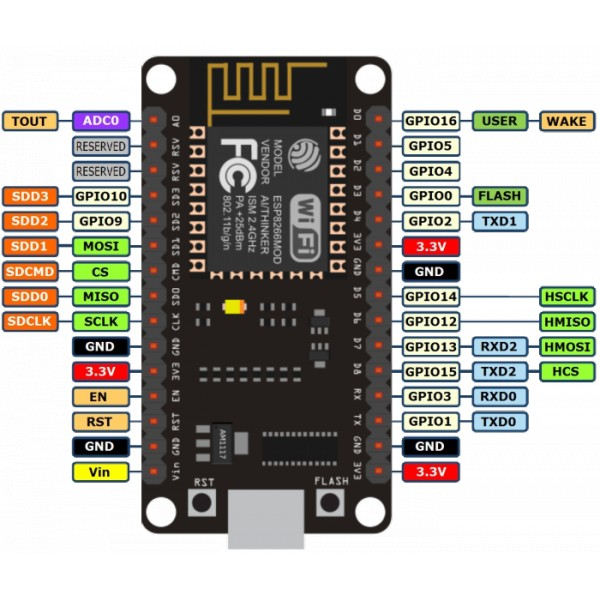
\includegraphics[scale=0.3]{nodemcu-v3-esp8266.jpg}
\caption{Node MCU( Esp8266)}
\end{figure}
ESP8266 no es un microcontrolador. Dentro si que lleva uno y se llama Tensilica L106 de 32-bit. La MCU se va a encargar de gestionar todas las entradas, salidas y cálculos necesarios para hacer funcionar el programa que hayamos cargado \cite{boylestad2003electronica}.
\begin{figure}[H]
\centering
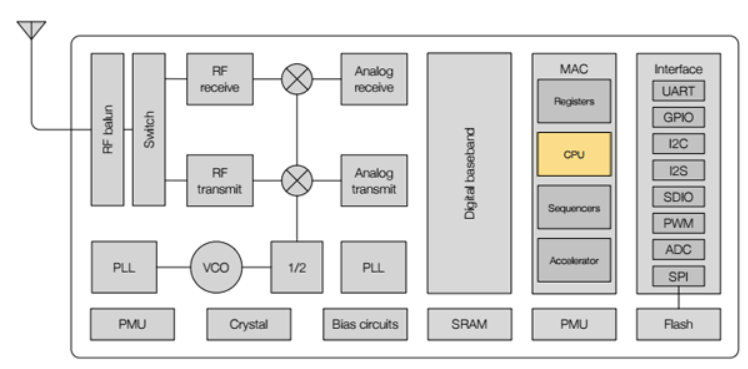
\includegraphics[scale=0.4]{8266.PNG}
\caption{ ESP8266EX Datasheet}
\end{figure}

\subsection{Sensor de PH}
El pH-4502C es una medida de acidez o alcalinidad de una disolución. El pH indica la concentración de iones hidronio [H3O+] presentes en determinadas sustancias. Este sensor permite medir el pH de un líquido mediante un electrodo ph y su placa controladora que ofrece un valor analógico proporcional a la medición.

\begin{figure}[H]
\centering
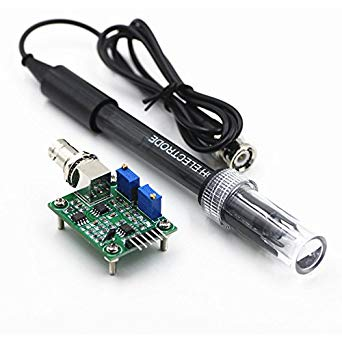
\includegraphics[scale=0.4]{ph1.jpg}
\caption{ Sensor module PH-4502C  }
\end{figure}

\subsection{Sensor de temperatura de agua}
El DS18B20 ofrece 9 a 12 bits lecturas de temperatura más una interfaz 1-Wire, por lo que sólo un hilo  debe conectarse desde un microprocesador central  con un voltaje de entrada 3.0 V-5.5 V y un rango de temperatura de -55   hasta + 125 grados centigrados \cite{kemmerly1975analisis}.
\begin{figure}[H]
\centering
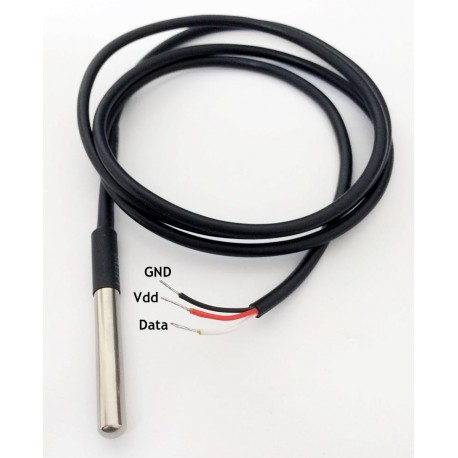
\includegraphics[scale=0.4]{sen_temp.jpg}
\caption{Sensor de temperatura DS18B20}
\end{figure}
\subsection{Sensor TDS conductividad}
TDS (total de sólidos disueltos): indica cuántos miligramos de sólidos disueltos se disuelven en 1 litro de agua. En general, cuanto mayor es el valor de TDS, más impura es el agua, posee un amplio suministro de voltaje de 3.3 ~ 5.5V y la salida de señal analógica de 0 ~ 2.3V.
\begin{figure}[H]
\centering
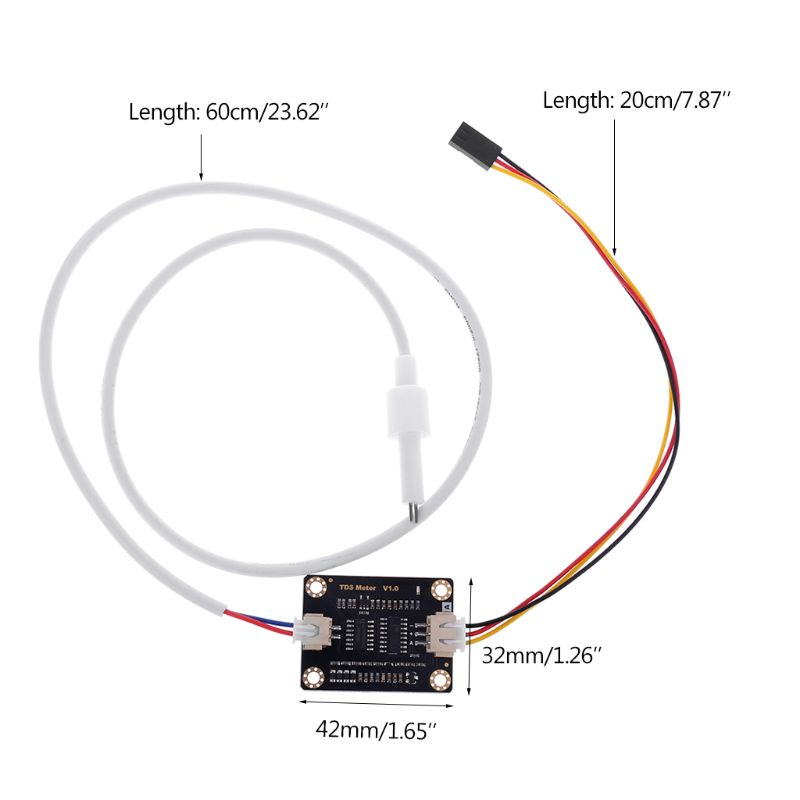
\includegraphics[scale=0.2]{TDS.jpg}
\caption{Sensor TDS}
\end{figure}
\subsection{Sensor de Turbidez (NTU)}
La turbidez es la medición de partículas en el agua. Este sensor de turbidez adopta un principio óptico para detectar la turbidez de la solución líquida,convierte la señal de corriente del sensor a voltaje de salida del módulo,cuanto menor es el voltaje de salida, mayor es el valor de turbidez. 
\begin{figure}[H]
\centering
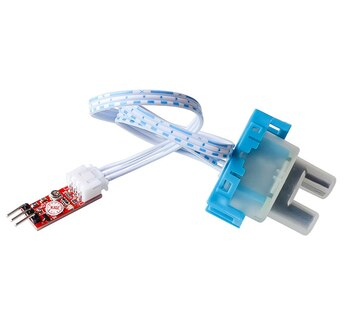
\includegraphics[scale=0.4]{TS-300B.jpg}
\caption{Sensor NTU }
\end{figure}

\end{multicols}
\section{Desarrollo}
\subsection{Diagrama de Bloques }
\begin{figure}[H]
\centering
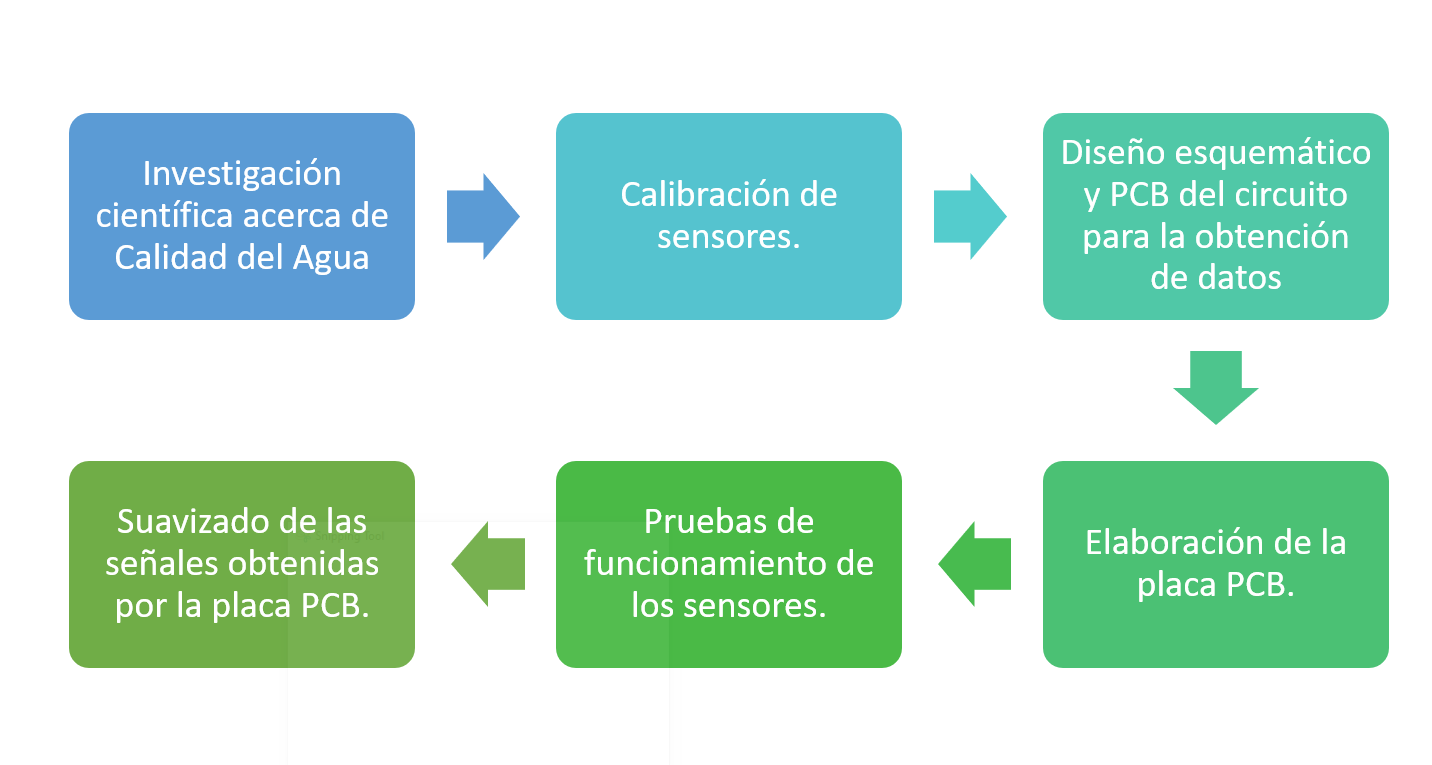
\includegraphics[scale=0.4]{diagrama.png}
\caption{Sensor NTU }
\end{figure}
\subsection{Calibración de sensores }
Los sensores utilizados para la obtención de datos sobre calidad del agua tienden a tener una alta precisión, y no todos funcionan de la misma manera, esto no significa que se usan métodos distintos de lectura, sino que la programación aplicada para la obtención de estos datos se basa en diferentes formulas y estrategias de calibración. A mayores, se cuenta con tres sensores analógicos y un sensor digital (temperatura - ver sección \ref{temp}).\\

Para la obtención de datos de nuestros sensores se ha diseñado una placa PCB con el circuito necesario para la interconexión de los mismos (ver sección \ref{pcb}) y se ha programado el código descrito en el Programa~\ref{lect}.

\lstinputlisting[language=Arduino, caption={Código utilizado para lectura de sensores}\label{lect}]{PrograSensor/LECTURA/LECTURA.ino}
\subsubsection{Calibración de Sensor de PH}
Para calibrar el sensor de PH  se toma en cuenta que el rango promedio de la sonda oscila entre valores negativos y positivos. El 0 representa un pH de 7.0. Para poder usarlo con Arduino, este circuito agrega un valor de compensación al valor medido por la sonda, por lo que el ADC solo tendrá que tomar muestras de valores de voltaje positivos. Por lo tanto, forzaremos un pH de 7.0 desconectando la sonda del circuito y cortocircuitando el interior del conector BNC con el exterior. Con un multímetro, mida el valor del  pin Po  y ajuste el potenciómetro para que sea 2,5$v$.\\

Tomando valores de tablas ya existentes de pH de diversos líquidos se va calibrando hasta tener unos similares.
\begin{figure}[H]
\centering
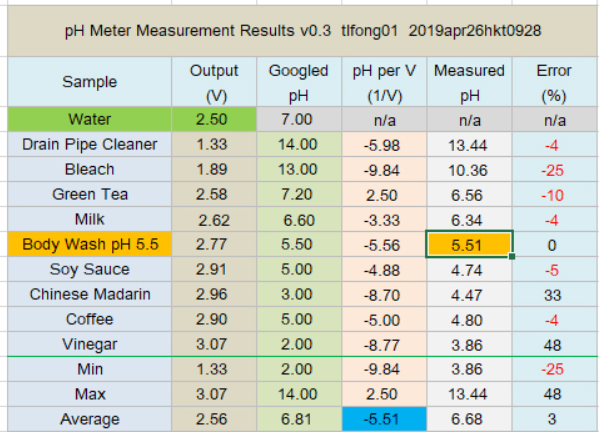
\includegraphics[scale=0.8]{tablaPH.PNG}
\caption{Tabla de pH}
\label{tabPH}
\end{figure}

Como se muestra en la Fig.~\ref{volt-ph}.  la gráfica resultante usando la fórmula general $y = mx + b$ se utiliza para calcular $x$ e $y$,donde  $x$  serían el voltaje y la $y$ el pH. El resultado es $ y = -5.70x + 21.34$.
\begin{figure}[H]
\centering
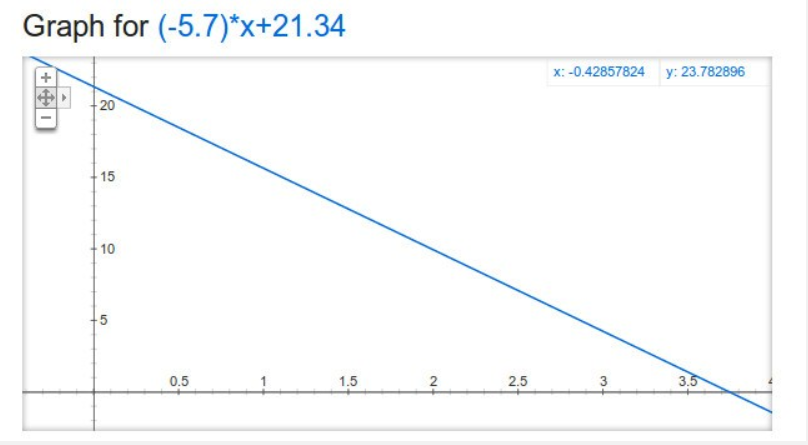
\includegraphics[scale=0.6]{calibradorPH.PNG}
\caption{Gráfica de relación voltaje-pH}
\label{volt-ph}
\end{figure}


\subsubsection*{Resultados obtenidos}
\begin{figure}[H]
\centering
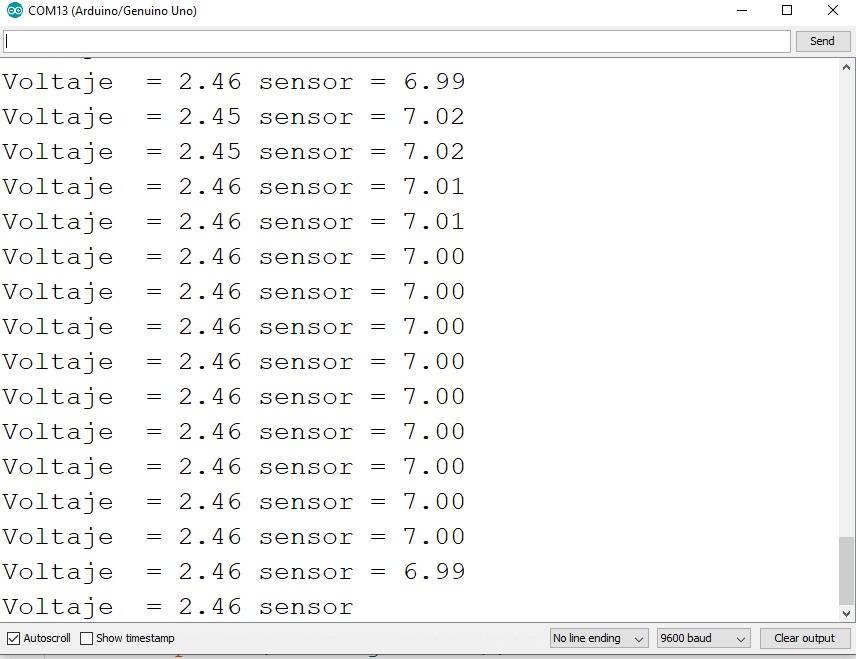
\includegraphics[scale=0.7]{Resultados/resPh}
\caption{Datos adquiridos de pH}
\end{figure}

\subsubsection{Calibración de Sensor de temperatura}\label{temp}
Para el sensor de temperatura se tomo muestras con agua de diferentes temperaturas, como el agua en 100 grados llega a su punto de ebullición
\begin{figure}[H]
\centering
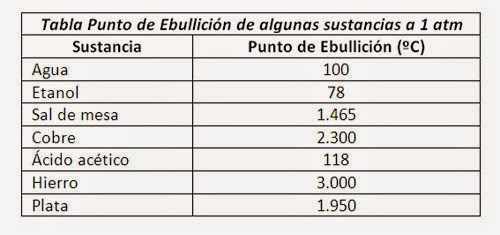
\includegraphics[scale=0.9]{ebullicion.jpg}
\caption{Punto de ebullición}
\end{figure}

\subsubsection*{Resultados obtenidos}
\begin{figure}[H]
\centering
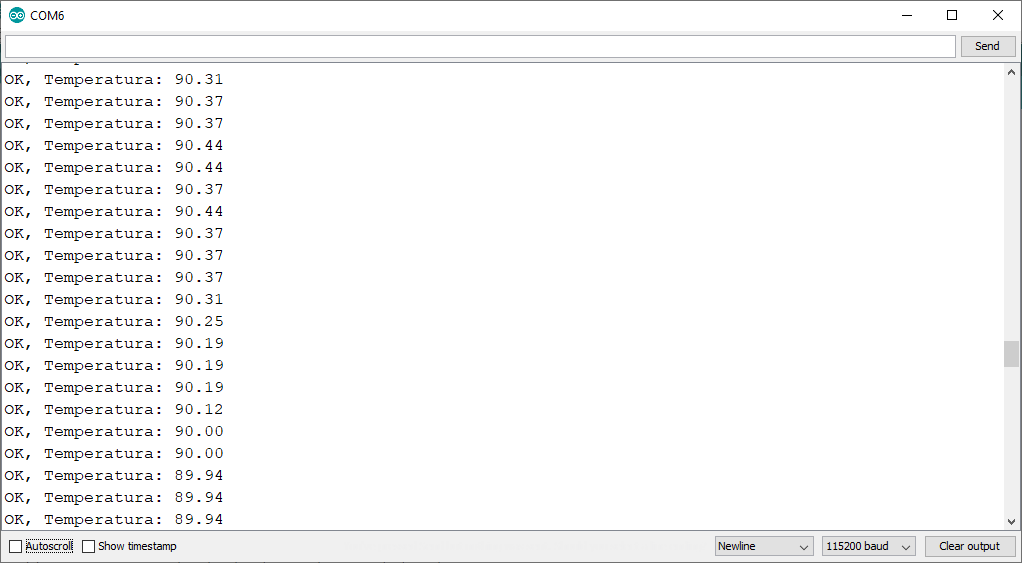
\includegraphics[scale=0.5]{Resultados/resTemperatura}
\caption{Datos adquiridos de Temperatura}
\end{figure}

\subsubsection{Calibración de Sensor TDS}
Tomando de referencia el color del agua se puede usar distintos colores de agua y tomando tablas ya existentes de referencia para calibrar el sensor.
\begin{figure}[H]
\centering
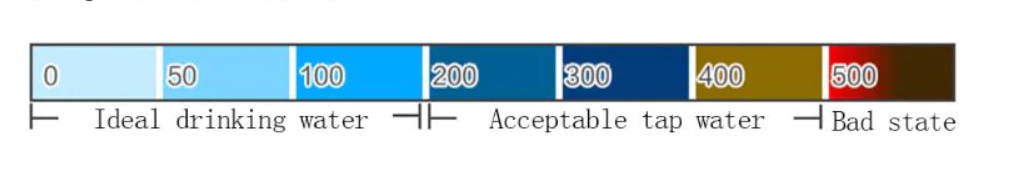
\includegraphics[scale=0.5]{turbidez.PNG}
\caption{Conductividad del agua}
\end{figure}

\subsubsection*{Resultados obtenidos}
\begin{figure}[H]
\centering
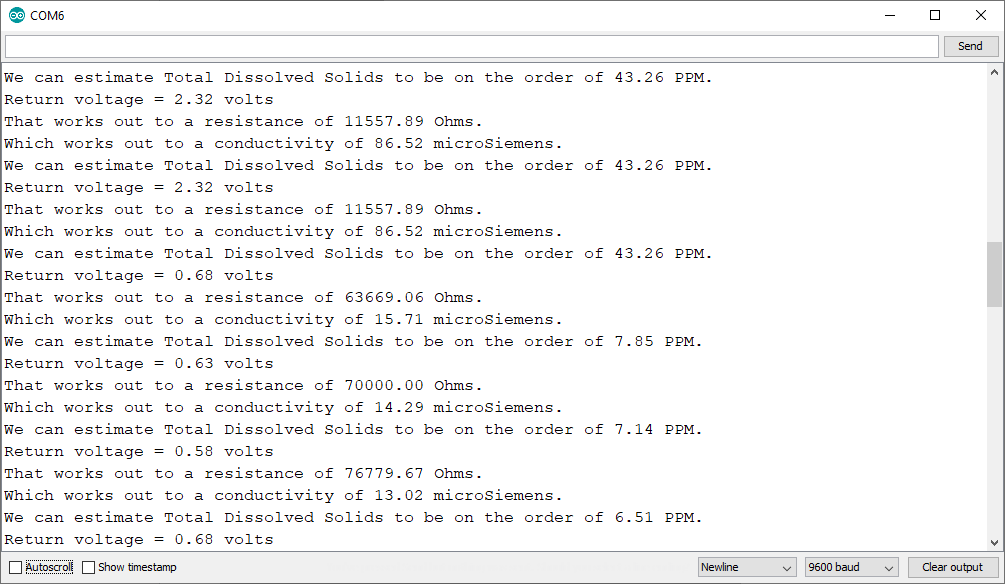
\includegraphics[scale=0.5]{Resultados/resTds}
\caption{Datos adquiridos de Calidad}
\end{figure}


\subsubsection{Calibración de Sensor NTU}
Ya que este módulo convierte la señal de corriente del sensor a voltaje de salida del módulo. Cuanto menor es el voltaje de salida, mayor es el valor de turbidez, y tomando como referencia para calibrar la turbidez en tablas ya existentes.
\begin{figure}[H]
\centering
\includegraphics[scale=0.4]{Turbidez.JPG}
\caption{Turbidez del agua dependiendo de la masa }
\end{figure}

\subsubsection*{Resultados obtenidos}
\begin{figure}[H]
\centering
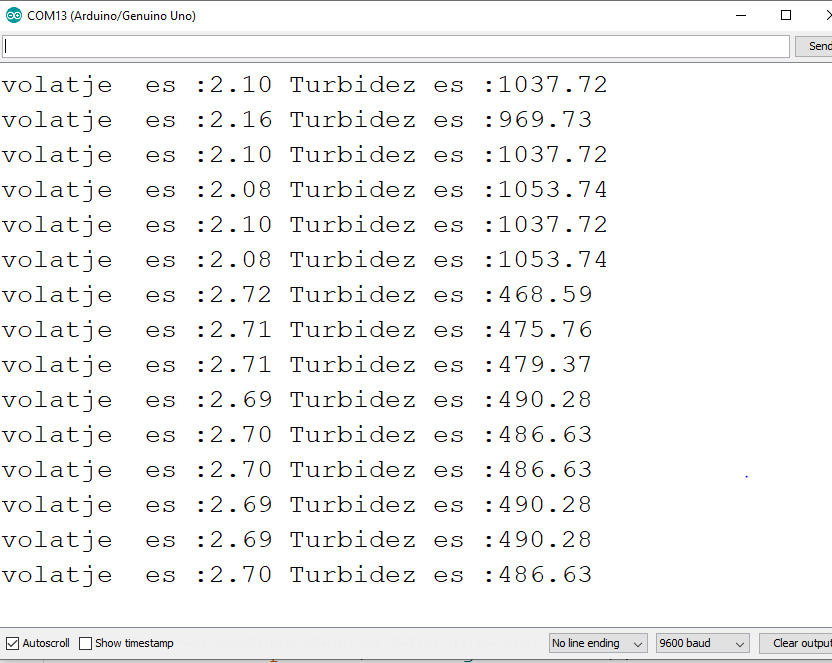
\includegraphics[scale=0.4]{Resultados/resTurbidez}
\caption{Datos adquiridos de Turbidez}
\end{figure}
\subsection{Diseño esquemático y PCB del circuito para la obtención de datos}\label{pcb}
Para el diseño se ha hecho uso de el software de diseño Eagle y el software de simulación y diseño Fritzing.
\subsubsection{Diseño del circuito en Eagle}
Para el diseño del circuito existen varios aspectos a tomar en cuenta:
\paragraph{NodeMCU v3} Este módulo posee un circuito integrado ESP8266MOD, es decir que tiene la posibilidad de conectarse a WiFi. El inconveniente es que este dispositivo únicamente cuenta con una entrada para la lectura de datos analógicos (pin A0); tomando en cuenta que se utiliza tres sensores analógicos es necesario el uso de un multiplexor analógico.
\paragraph{CJMCU-4051} Es el componente que se encarga de convertir la única entrada analógica del NodeMCU en ocho distintas, utilizando el circuito integrado 74HC4051. Cabe recalcar que en el software Eagle no existe este elemento, ni existe una librería que facilite la manipulación de este, por este motivo se lleva a cabo la creación de la misma.
\paragraph{Sensores} Los sensores utilizados son conectados a distintos mólex de 3 pines para facilitar su enlace a la placa y no tener errores de polaridad.
\paragraph{Componentes extras} El sistema además cuenta con dos LEDs indicadores, un pulsador de uso multipropósito y un conector DC hembra que se encargará de alimentar el circuito completo con una fuente externa de 5v.

\subsubsection*{Diseño de librería para el CJMCU-4051}
Se procede a diseñar una librería que proporcione las dimensiones necesarias para la implementación del CJMCU-4051 en el software Eagle.
\begin{figure}[H]
\centering
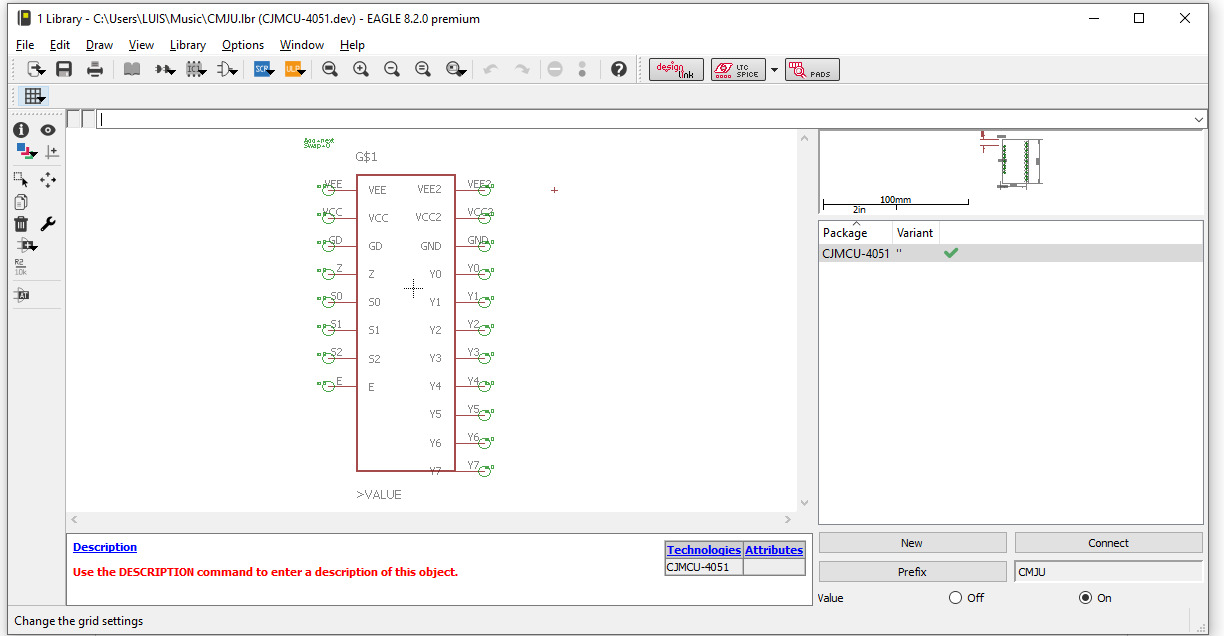
\includegraphics[scale=0.4]{mux1.jpeg}
\caption{Diseño de componente esquemático}
\end{figure}
\begin{figure}[H]
\centering
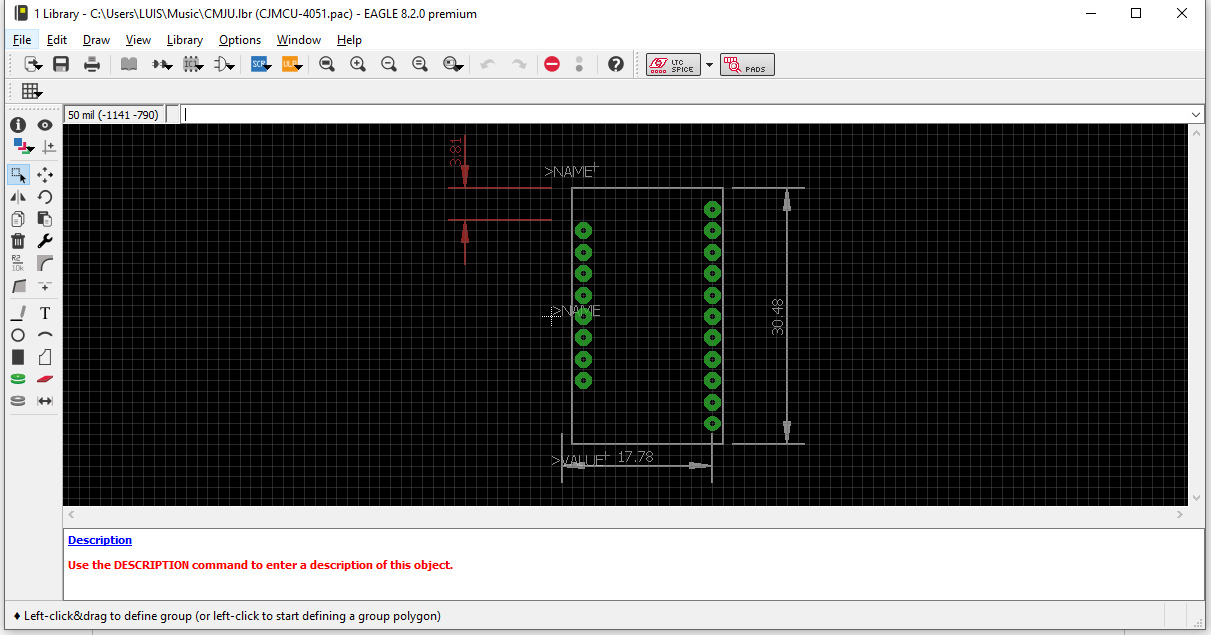
\includegraphics[scale=0.4]{mux3.jpeg}
\caption{Diseño de componente PCB}
\end{figure}

A continuación, se ubican todos los elementos en el espacio de trabajo y se procede a diseñar el esquemático, obteniendo el resultado mostrado en la Fig.~\ref{esquematic}.
\begin{figure}[H]
\centering
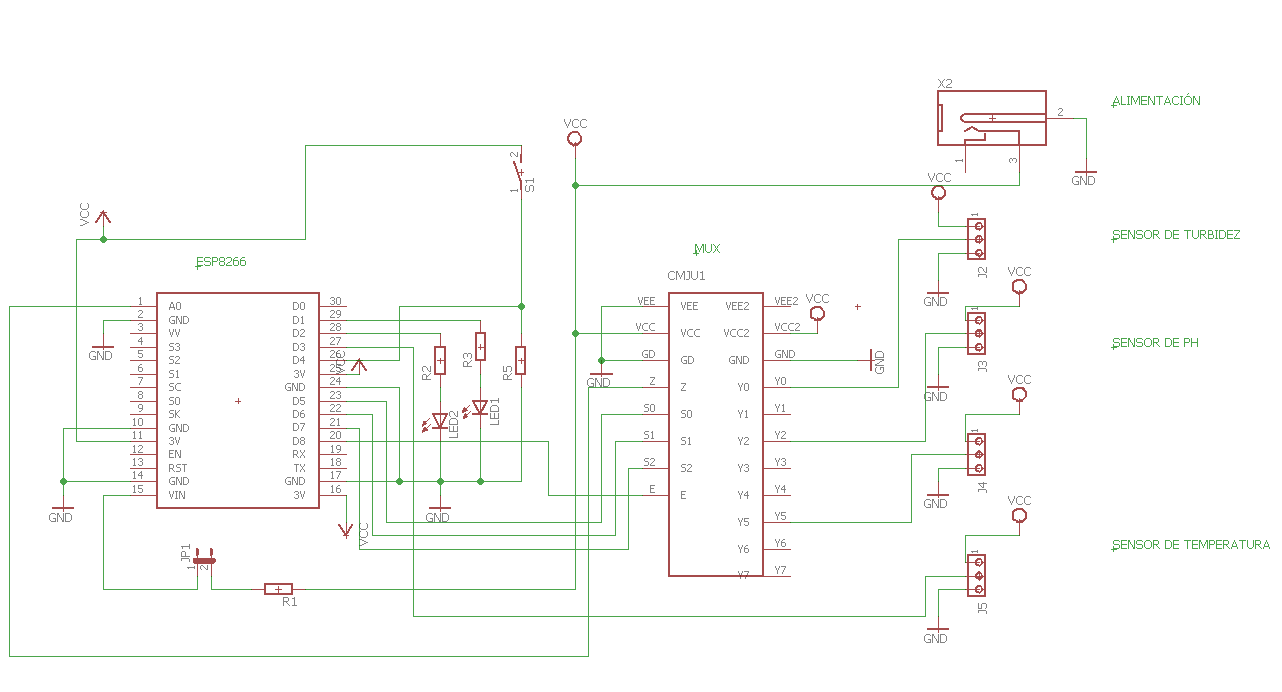
\includegraphics[scale=0.48]{eagle.png}
\caption{Diseño de esquemático del circuito}
\label{esquematic}
\end{figure}

Por último, se procede a diseñar el PCB en Eagle teniendo como resultado la Fig.~\ref{pcb_Eagle}.

\begin{figure}[H]
\centering
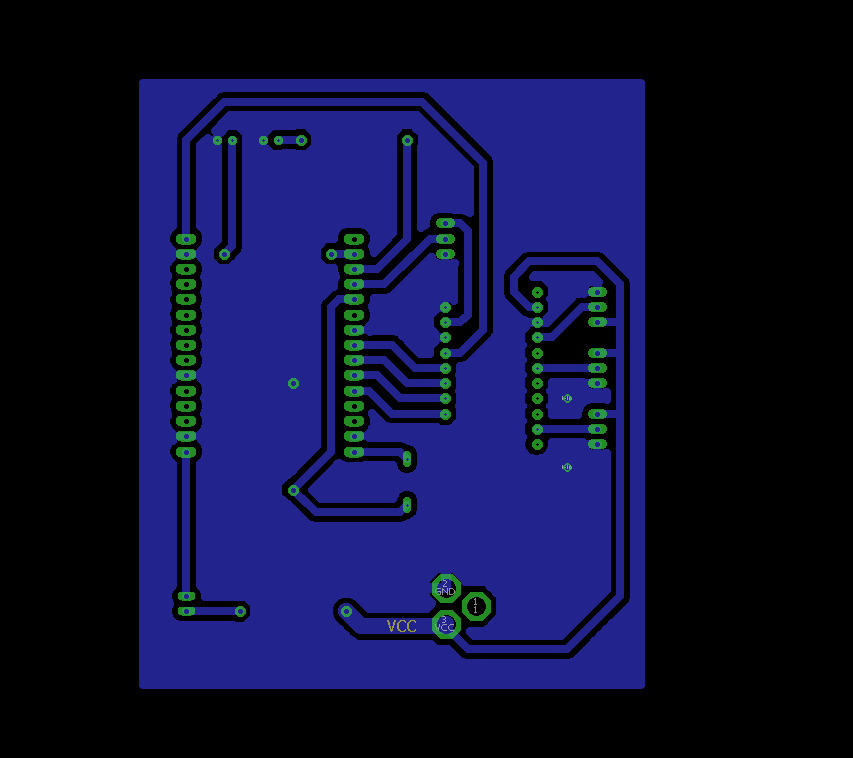
\includegraphics[scale=0.35]{pcb_eagle}
\caption{Diseño de PCB del circuito}
\label{pcb_Eagle}
\end{figure}


\subsubsection{Diseño del circuito en Fritzing}
Los elementos del circuito se colocan tal y como quedaran si están sobre una protoboard.

\begin{figure}[H]
\centering
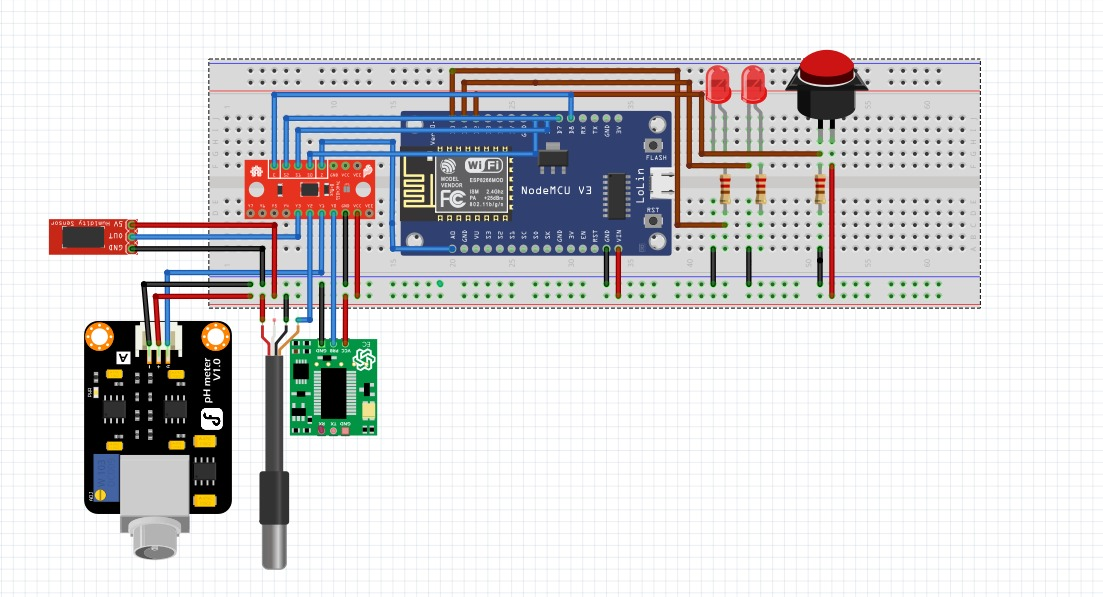
\includegraphics[scale=0.40]{fritzing}
\caption{Armado en protoboard usando Fritzing}
\end{figure}
\subsubsection{Elaboración de la placa PCB}
Una vez el diseño esté terminado se imprime en papel transferible o papel fotografía y se plancha en la placa de cobre para que el diseño se transfiera.
\begin{figure}[H]
\centering
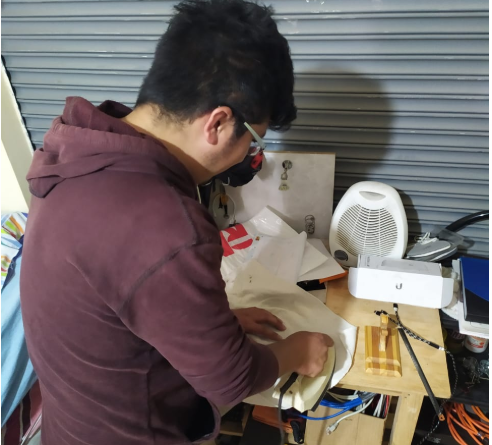
\includegraphics[scale=0.6]{planchado}
\caption{Planchado de placa de cobre }
\end{figure}

Con ayuda de ácido de Percloruro de Hierro se quema la placa y así se obtiene el diseño que se imprimió en la placa
\begin{figure}[H]
\centering
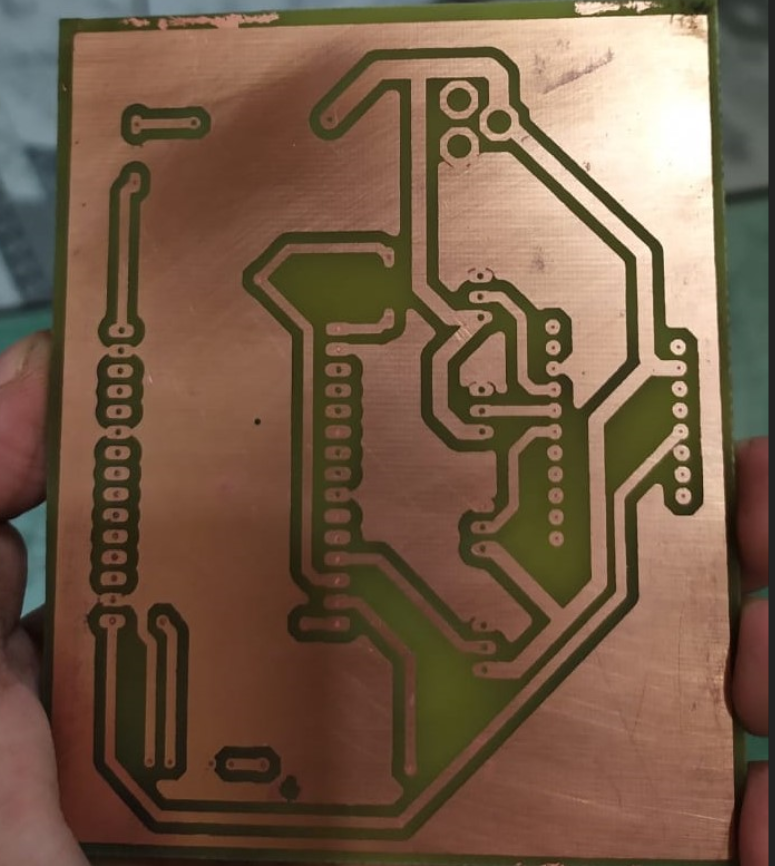
\includegraphics[scale=0.3]{placa}
\caption{Placa PCB perforada}
\end{figure}

Se ubica los elementos en su lugar y se procede a soldar.
\begin{figure}[H]
\centering
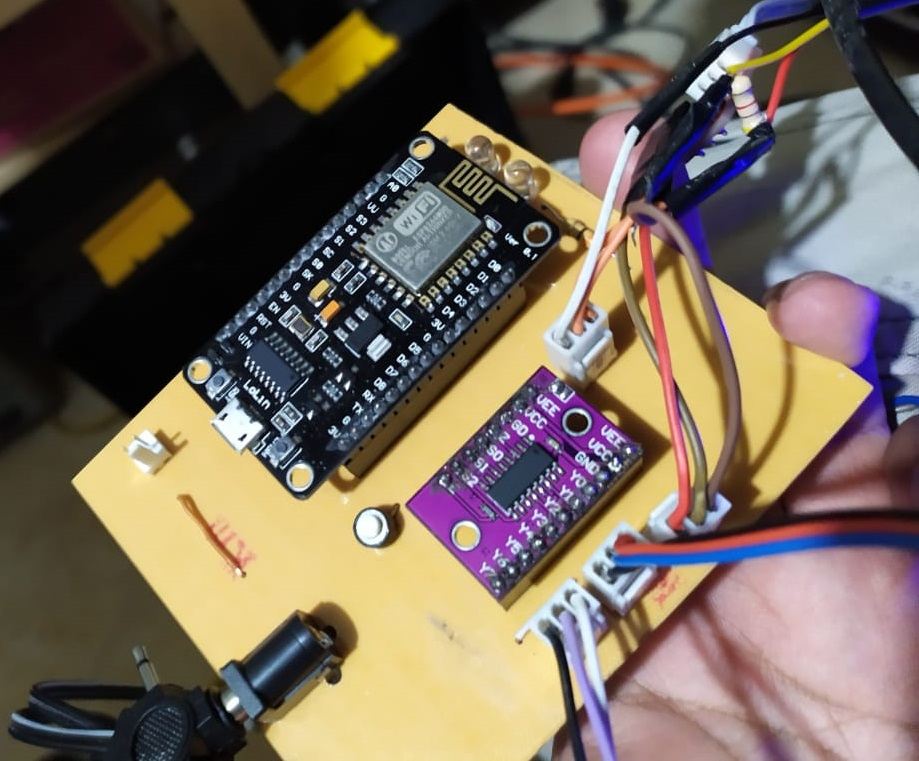
\includegraphics[scale=0.3]{todo}
\caption{Placa terminada }
\end{figure}

Para verificar el correcto funcionamiento de la placa PBC se procede a hacer las pruebas pertinentes.
\begin{figure}[H]
\centering
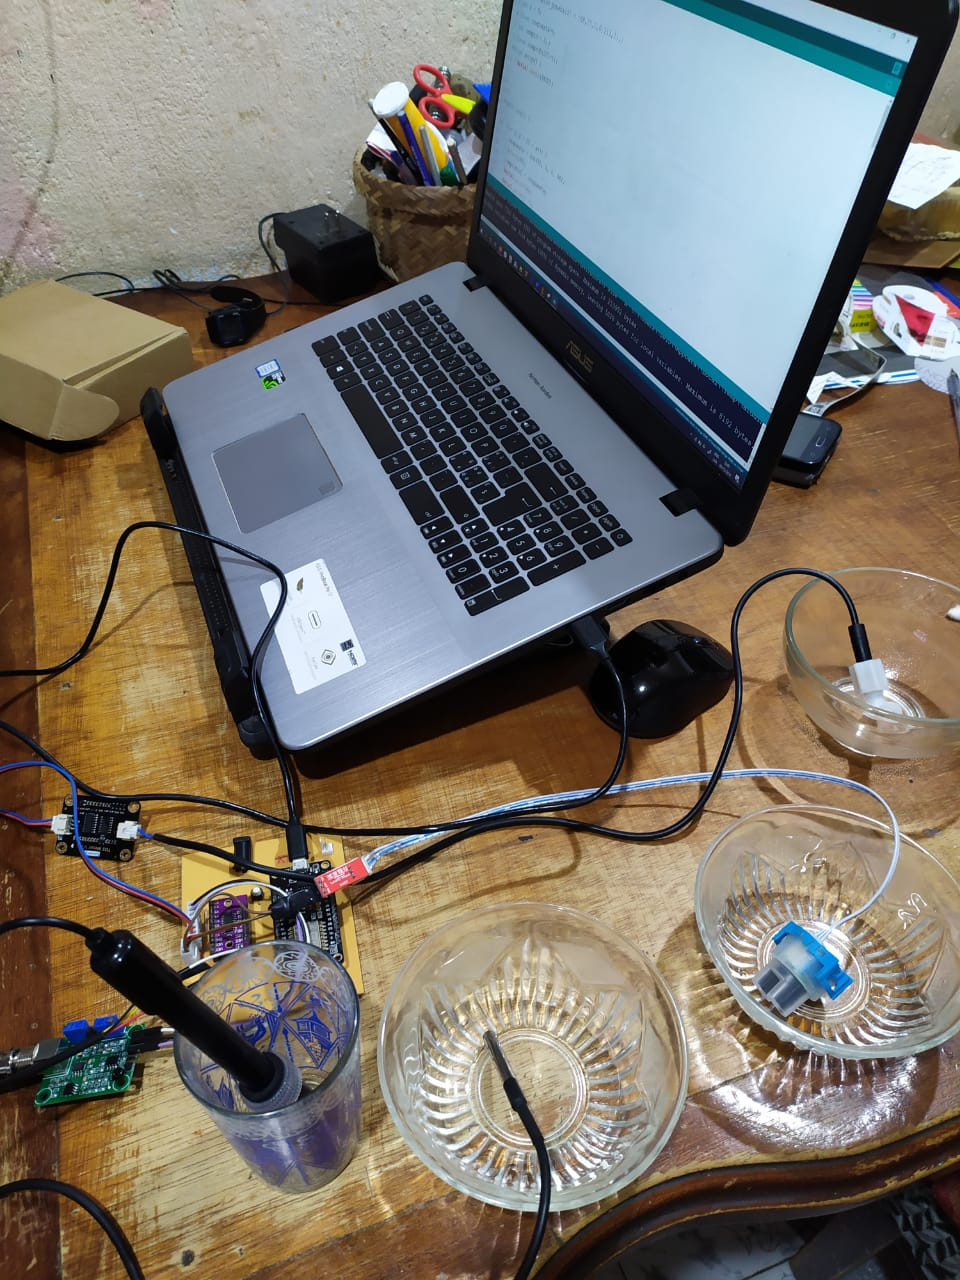
\includegraphics[scale=0.2]{muestras}
\caption{Toma de datos}
\end{figure}
\subsection{Toma de datos}
Se obtiene una base de datos almacenada en una matriz de 120 filas por 20 columnas, utilizando el Programa~\ref{lect}; estos datos obtenidos en el Monitor Serial se copian a un nuevo libro de Excel y utilizando la herramienta \lstinline!CONCAT! ordenamos los valores de modo que tengan la sintaxis de una matriz (Fig.~\ref{excel}).

\begin{figure}[H]
\centering
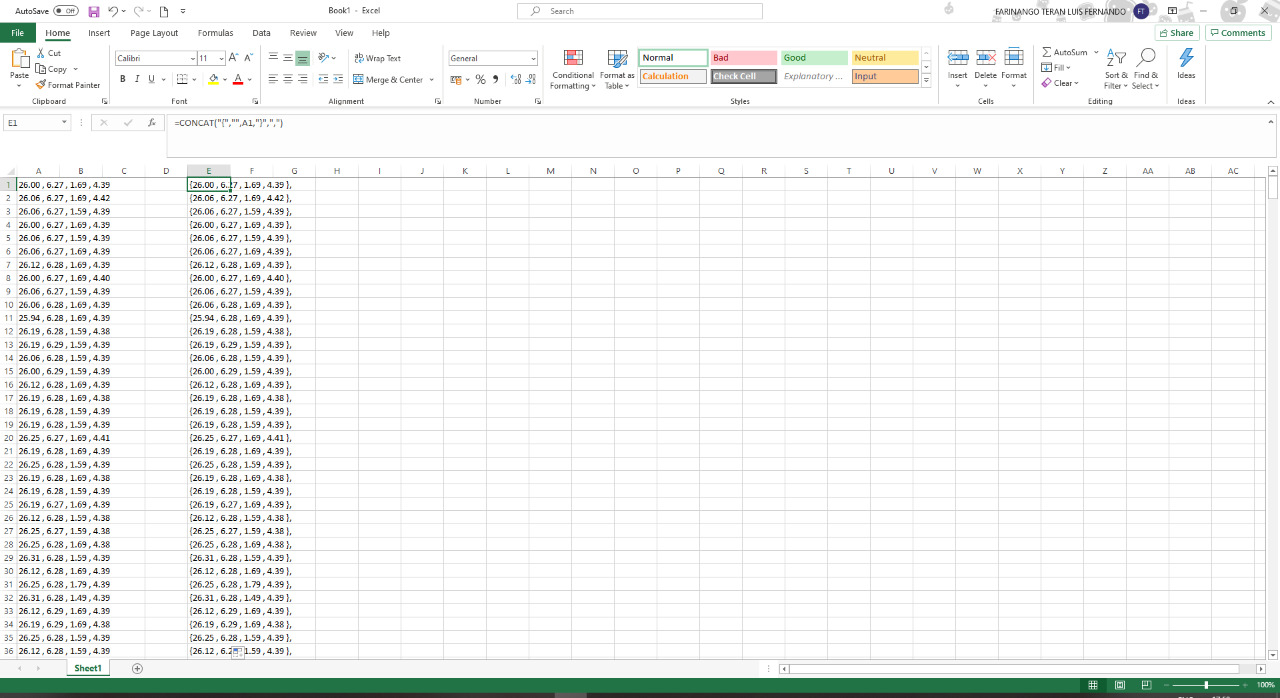
\includegraphics[scale=0.35]{excel}
\caption{Concatenación de datos}
\label{excel}
\end{figure}

\subsection{Suavizado de datos mediante algoritmos matemáticos}

\subsubsection{Algoritmo de Kalman}
El filtro discreto de Kalman se basa en la estimación de un estado x en un tiempo discreto. El filtro de Kalman proporciona un buen marco para la estimación incremental de una cantidad en una situación en la cual las mediciones relacionadas con la misma están disponibles a lo largo del tiempo. Concretamente, se trata de una técnica de estimación Bayesiana empleada para seguir sistemas estocásticos dinámicos observados mediante sensores ruidosos. El filtro es un procedimiento matemático que opera por medio de un mecanismo de predicción y corrección.  En esencia este algoritmo pronostica el nuevo estado a partir de su estimación previa añadiendo un término de corrección proporcional al error de predicción, de tal forma que este último es minimizado estadísticamente

En el paso de predicción la estimación del estado se calcula con la siguiente ecuación: 
\begin{equation}
\hat{x}^{-}_{k} = A \cdot \hat{x}_{k-1} + B \cdot \mathcal{U}_{k-1}
\end{equation}
donde $\hat{x}^{-}_{k}$ es el estado observado en el paso de tiempo $k$, $\mathcal{U}_{k-1}$ es una entrada de control en el paso de tiempo $k-1$ al estado en el paso de tiempo $k$ \cite{Kowalski2018}. En la siguiente etapa de el paso de predicción, el calculo de la proyección de covarianza de error se debe realizar con la siguiente fórmula:
\begin{equation}
P^{-}_{k} = A \cdot P_{k-1} + A^T + Q
\end{equation}
donde $P^{-}_{k}$ es la covarianza de error que es estimada \textit{a priori}, $P_{k-1}$ es la covarianza de error que es estimada \textit{a posteriori} y $Q_{n \times n}$ el error de proceso (covarianza de ruido) \cite{Kowalski2018}.

La ganancia de Kalman es calculada con la siguiente fórmula:
\begin{equation}
K_{k} = P^{-}_{k} \cdot H^T \cdot (H\cdot P^-_{k}+R)^{-1}
\end{equation}

donde la matriz $H$ demuestra la medición con el estado $x$. La matriz $R$ es la precisión de la medición. Finalmente, la fórmula para la estimación de estado pasaría a ser
\begin{equation}
\hat{x}_{k} = \hat{x}^{-}_{k} + K_{k} \cdot (z_k - H \cdot \hat{x}^{-}_{k})
\end{equation}

donde $\hat{x}_{k}$ es la estimación del estado a posteriori, $\hat{x}^{-}_{k}$ es el estado observado en el tiempo de paso $k$, $K_{k}$ es la ganancia que controla la influencia de la medición en $\hat{x}_{k}$, $\hat{z}_{k}$ es la medición en el tiempo de paso $k$ y la matriz $H$ da la relación de la medición al estado \cite{Kowalski2018}.

Al final del procedimiento la actualización de covarianza de error es requerida. Su fórmula es la siguiente:
 
\begin{equation}
P_{k} = (I - K_{k} \cdot H) \cdot P^{-}_{k}
\end{equation}

Teniendo esta teoría presente procedemos a programar el código en la plataforma de Arduino IDE, obteniendo el resultado planteado en el Programa~\ref{pro_kalman}.

\lstinputlisting[language=Arduino, caption={Código del filtro Kalman}\label{pro_kalman}]{PrograSensor/kalman/kalman.ino}

\subsubsection{Algoritmo Median}
Es un filtro no lineal que suaviza el impulso del ruido sin disminuir la amplitud en la señal, usado para reducir el ruido aleatorio cuando la amplitud del ruido tiene colas grandes y patrones periódicos. Donde se calcula la mediana de los valores y se la ubica en el centro de la ventana de entrada.

\begin{equation}
z_{j} = median(x_{j-n} .. x_{j-2}, x_{j-1}, x_{j+1}, x_{j+2} .. x_{j+n})
\end{equation}

Con el propósito de encontrar la mediana, 

\begin{equation}\label{eq_median}
\left \{ \begin{matrix} S_{(N+1)/2} & \mbox{, si }N mod \ 2 == 1\\
\displaystyle\frac{S_{N/2-1}+ S_{N/2+1}}{2} & \mbox{, si }N mod \ 2==0\end{matrix}\right.
\end{equation}

La formula~\ref{eq_median} describe la selección de la mediana de la lista ordenada $S$. Si $N$ es impar, la mediana es la muestra $S_{(N+1)/2}$, sino la media es el promedio de dos elementos $S_{N/2-1}$ y $S_{N/2+1}$ \cite{Kowalski2018}.\\

A continuación se detalla la manera en la que se programa este tipo de filtros.

\lstinputlisting[language=Arduino, caption={Código del filtro Median}\label{pro_median}]{PrograSensor/median_filter/median_filter.ino}

\subsubsection{Algoritmo Mean}
El filtrado medio es un método para suavizar la señal, es decir reduce la cantidad de variación de intensidad entre un dato y el otro, calculando el promedio de todas las muestras de su ventana.\\

El valor de salida es calculado computando el promedio de todas las muestras de la ventana. Su fórmula tiene la forma detallada a continuación:

\begin{equation}
z_j = \displaystyle\frac{\displaystyle\sum_{i=-n}^n x_{j+i}}{2n+1}
\end{equation}

donde $x_i$ es una muestra de la señal de entrada, $2n+1$ es la longitud de la ventana, $z_j$ representa el valor de salida, y $j$ es el índice actual de el valor de salida.\\

El código elaborado para evidenciar este filtro es bastante sencillo, se puede observar en el Programa~\ref{pro_mean}.

\lstinputlisting[language=Arduino, caption={Código del filtro Mean}\label{pro_mean}]{PrograSensor/Mean_Filter/Mean_Filter.ino}


\subsection{Resultados del suavizado de datos}
\subsubsection{Algoritmo de Kalman}

\begin{figure}[H]
\centering
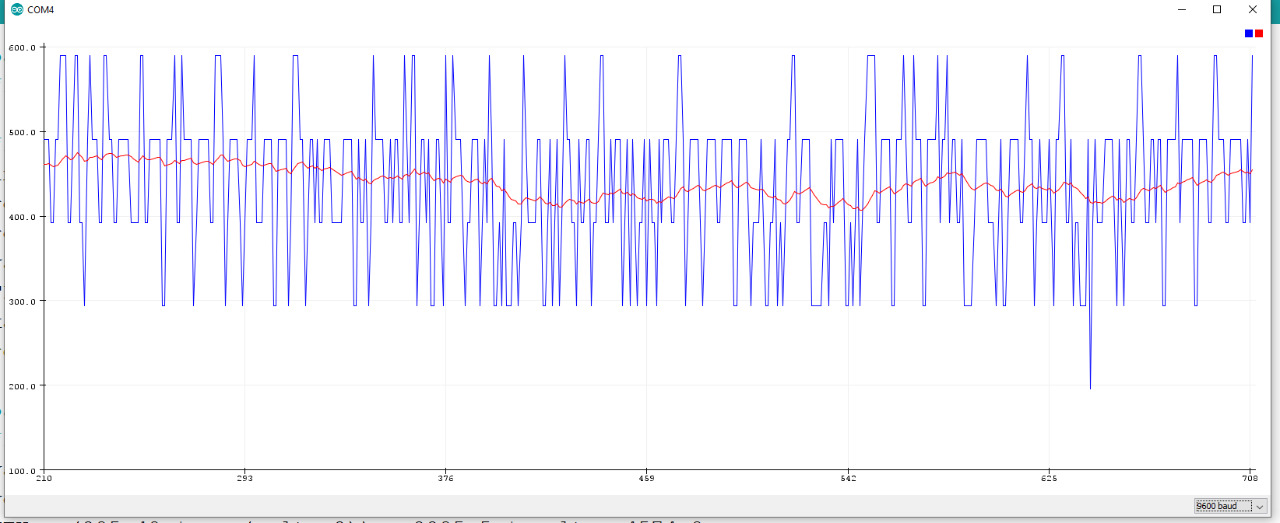
\includegraphics[scale=0.3]{kalman}
\caption{Suavizado con Filtro Kalman}
\end{figure}

\subsubsection{Algoritmo Median}
\begin{figure}[H]
\centering
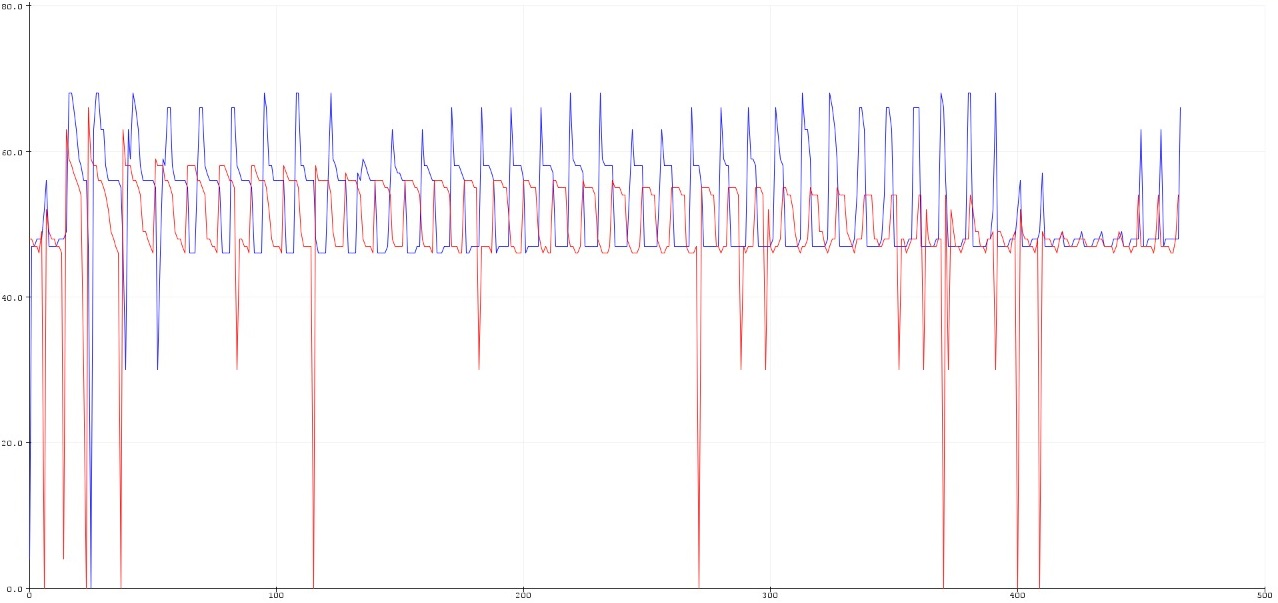
\includegraphics[scale=0.35]{median}
\caption{Suavizado con Filtro Median}
\end{figure}

\subsubsection{Algoritmo Mean}
\begin{figure}[H]
\centering
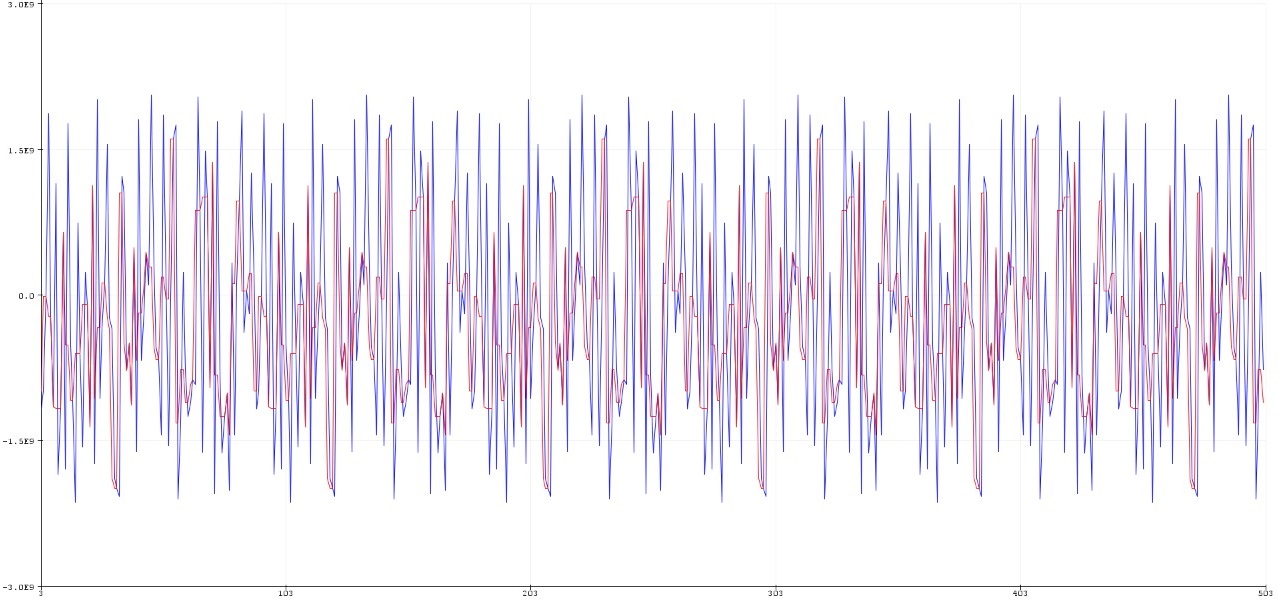
\includegraphics[scale=0.35]{mean}
\caption{Suavizado con Filtro Mean}
\end{figure}

\subsection{Errores}
Para el cálculo de errores se ha tomado en cuenta la presencia de ruido en los datos generados en forma de matriz ,cada columna de la matriz corresponde a la señal de un sensor. Por lo que utiliza tres tipos de error :erro relativo ,error absoluto y error cuadrático medio .
El error absoluto se guarda en una matriz de errores dado que dicho error se calcula en cada una de las mediciones de cada uno de los sensores ,de igual forma se crea una matriz de error relativo que hará la misma tarea de la matriz de error absoluto. Para el calculo de los dos errores antes mencionados se tiene en cuenta una consideración ,se debe tener un valor considerado como esperado .
Este valor se puede conseguir directamente de la medición o como la formula para el calculo de dicho error .Para este caso ,los errores son mas altos en el sensor de PH dado que es el que mayor variación de voltaje tiene en la señal obtenida.
Para el calculo del MSE ,se realiza un proceso parecido a diferencia que en este error ya se tiene una ecuación definida para calcularlo. Este tipo de error se usa cuando se tiene dos conjuntos de datos y necesita un valor previsto y un valor observado pero en este caso se usa una estimación del valor a obtener, por ejemplo se espera que el valor de temperatura de la muestra sea de aproximadamente 32 grados Celsius .
De acuerdo a los resultados se obtiene que el mayor MSE sigue correspondiendo al del sensor de PH, este tipo de error solo devuelve un único valor a diferencia de los errores absoluto y relativo que abarcan a cada una de las mediciones.
\begin{figure}[H]
\centering
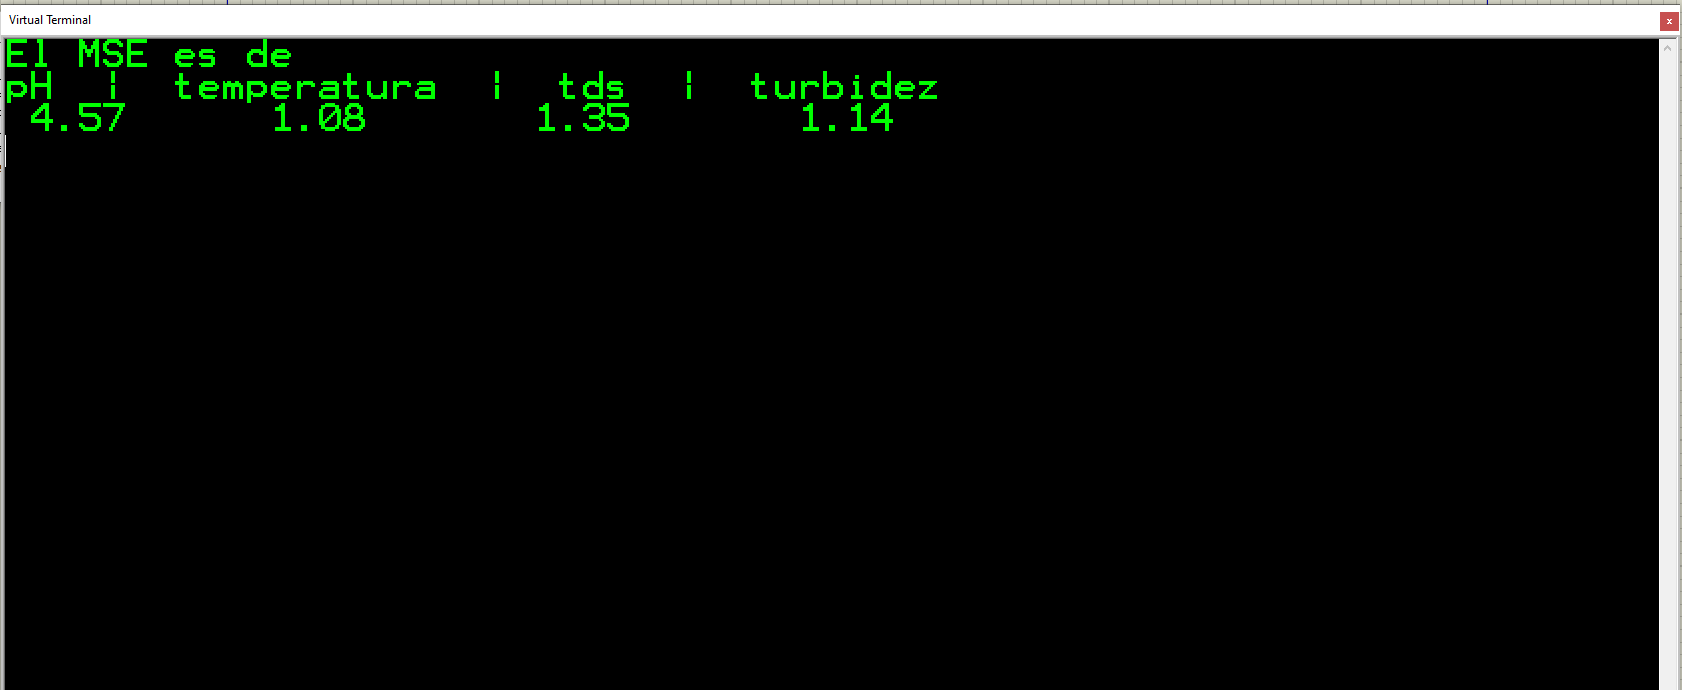
\includegraphics[scale=0.30]{MSE.png}
\end{figure}
\begin{figure}[H]
\centering
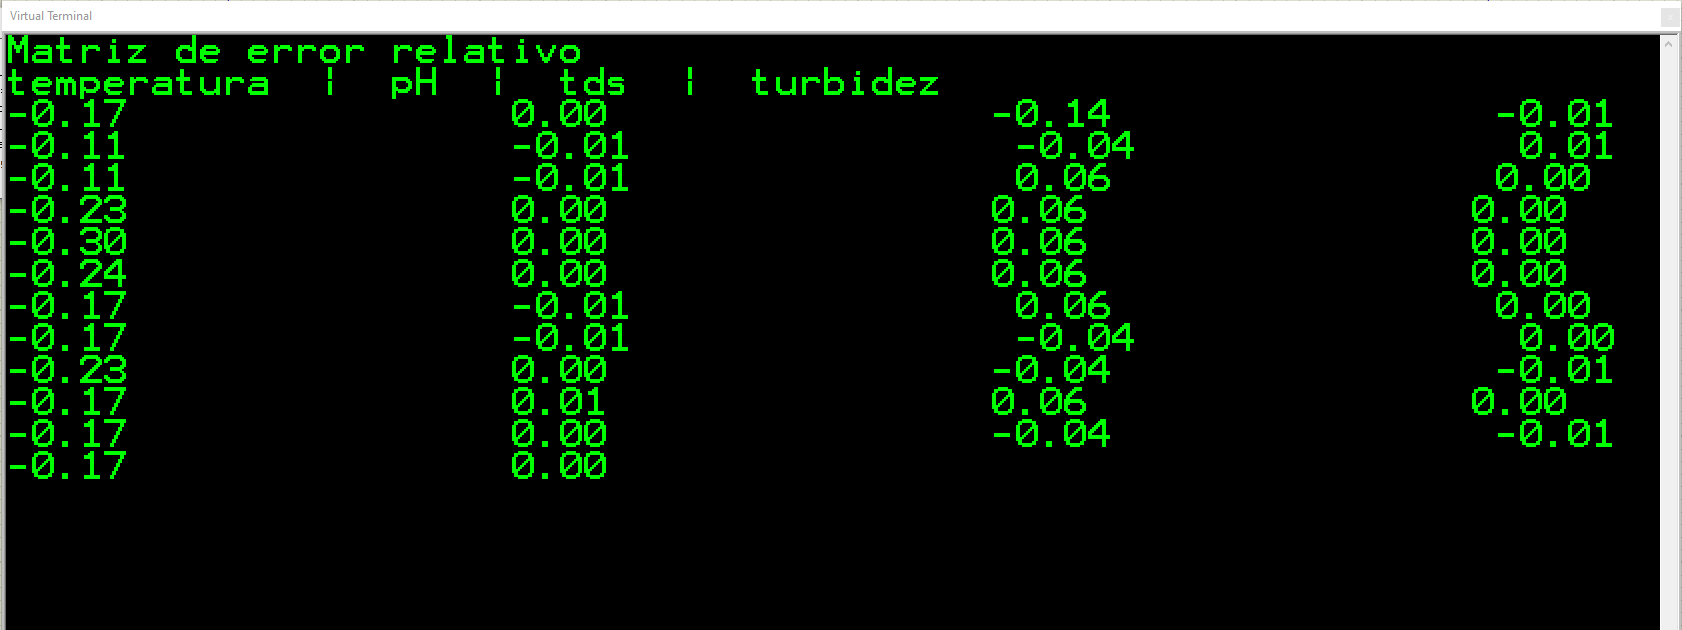
\includegraphics[scale=0.30]{Errorabsrlt.png}
\caption{Errores resultantes }
\end{figure}
\subsection{Relación Señal Ruido}
Para el cálculo de la relación señal ruido se puede realizar el siguiente proceso con cualquiera de los filtros de suavizado utilizados .Se resta la señal filtrada con la señal original ,el resultado será el ruido. A continuación, se divide la señal con el ruido obtenido .
\begin{figure}[H]
\centering
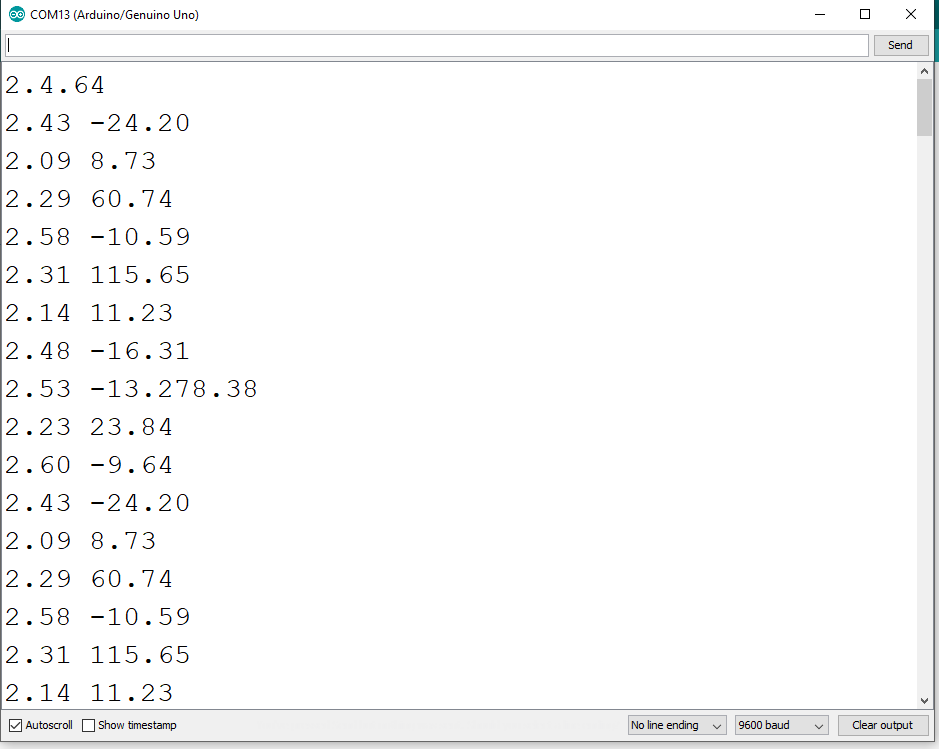
\includegraphics[scale=0.35]{snr.png}
\caption{datos de SNR(izquierda) y señal(derecha)}
\end{figure}
\begin{figure}[H]
\centering
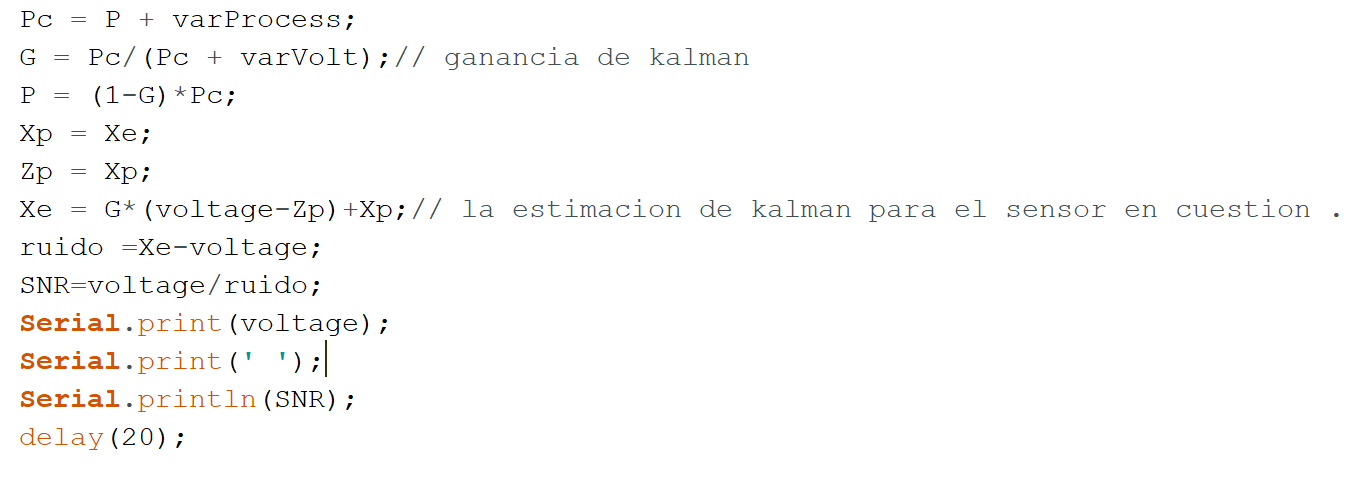
\includegraphics[scale=0.35]{snr2.png}
\caption{SNR en codigo de arduino}
\end{figure}
\begin{figure}[H]
\centering
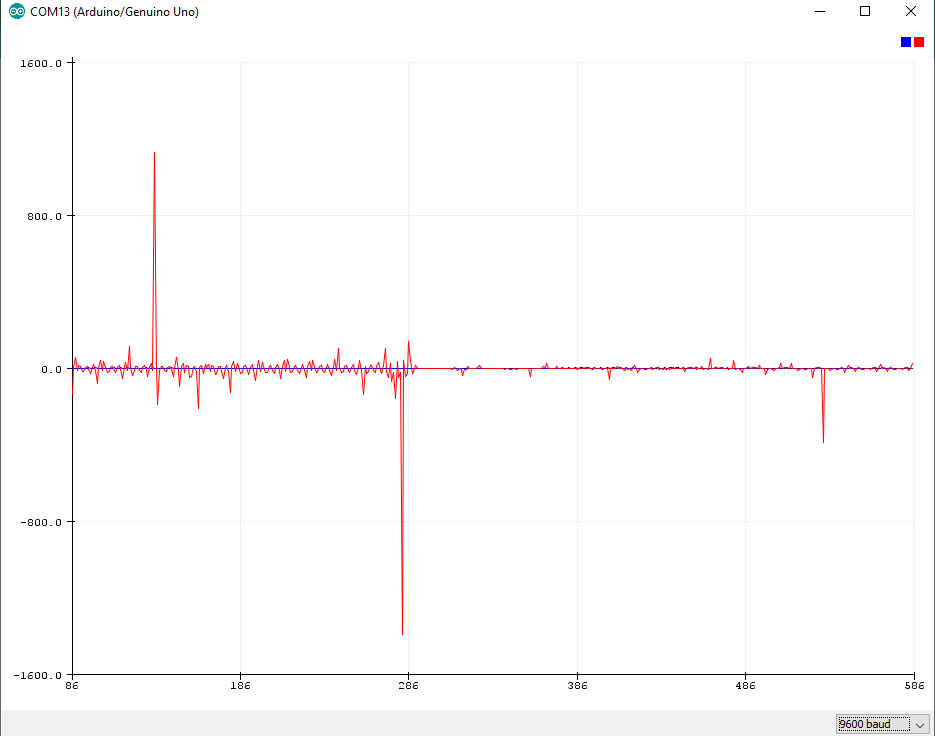
\includegraphics[scale=0.35]{snr3.png}
\caption{SNR en plotter de arduino}
\end{figure}
\section{Análisis de Resultados}
En base a las graficas obtenidas se tiene que Mediam filter presenta una reducción en los puntos máximos que se podrían considerar como ruido y de esta forma el suavizado, pero presenta unos picos altos cuando llega al punto medio. Mean filter presenta un suavizado significativo de los picos más altos, pero es casi no muy relevante ya que el suavizado no es muy prolongado. Karnalm filter se pudo apreciar que este filtro es el que mejor resultado presento, el suavizado que mostro ante los picos de ruido fue más relevante en comparación con los otros, trabajado de mejor manera ante la reducción de los picos.
\section{Conclusiones y Recomendaciones}

\subsection*{Conclusiones}
\begin{itemize}
\item La conductividad del agua depende estrictamente de cuanto se encuentre contaminada ya que una mayor contaminación se traduce como una mayor cantidad de impurezas en el líquido, esto provoca una concentración de iones que hacen que la conductividad aumente.   
\item La calibración del sensor de turbidez y pH esta basado en ecuaciones que dan la relación de estas dos magnitudes en función del voltaje.
\item El uso del componente electrónico ESP8266(NodeMCU) puede llegar a dar un sinnúmero de problemas, ya que no es un dispositivo utilizado muy a menudo y es complicado encontrar información acerca de este y de su funcionamiento, a mayores, este MCU cuenta con incompatibilidades con ciertas librerías de arduino, pero siempre se encuentra otra alternativa.
\item Generar una base de datos muy amplia provoca que la CPU del microcontrolador se sature y por ende, no rinda con los resultados deseados; a mayores, utilizar un algoritmo en tiempo real, es decir de manera continua, provoca un gran esfuerzo por parte del dispositivo, pero no consume tanto rendimiento del mismo.
\end{itemize}

\subsection*{Recomendaciones}
\begin{itemize}
\renewcommand{\labelitemi}{$*$}
\item Calibrar los sensores con un número de muestras amplia, ya que así se puede comprobar el correcto funcionamiento de dichos sensores.
\item Revisar el datasheet para saber cual es el valor de alimentación de trabajo de los sensores para no averiarlos.
\item Encontrar las ecuaciones adecuadas para cada calibración, existirán casos donde se deberá generar la ecuación en base a mediciones de los sensores.
\item Se debe realizar la obtención de los datos cuando los sensores se encuentran con una lectura estable con el propósito de que los valores conseguidos no cambien abruptamente en muestras continuas.
\end{itemize}

\section{Anexos }
\begin{multicols}{2}
\begin{figure}[H]
\centering
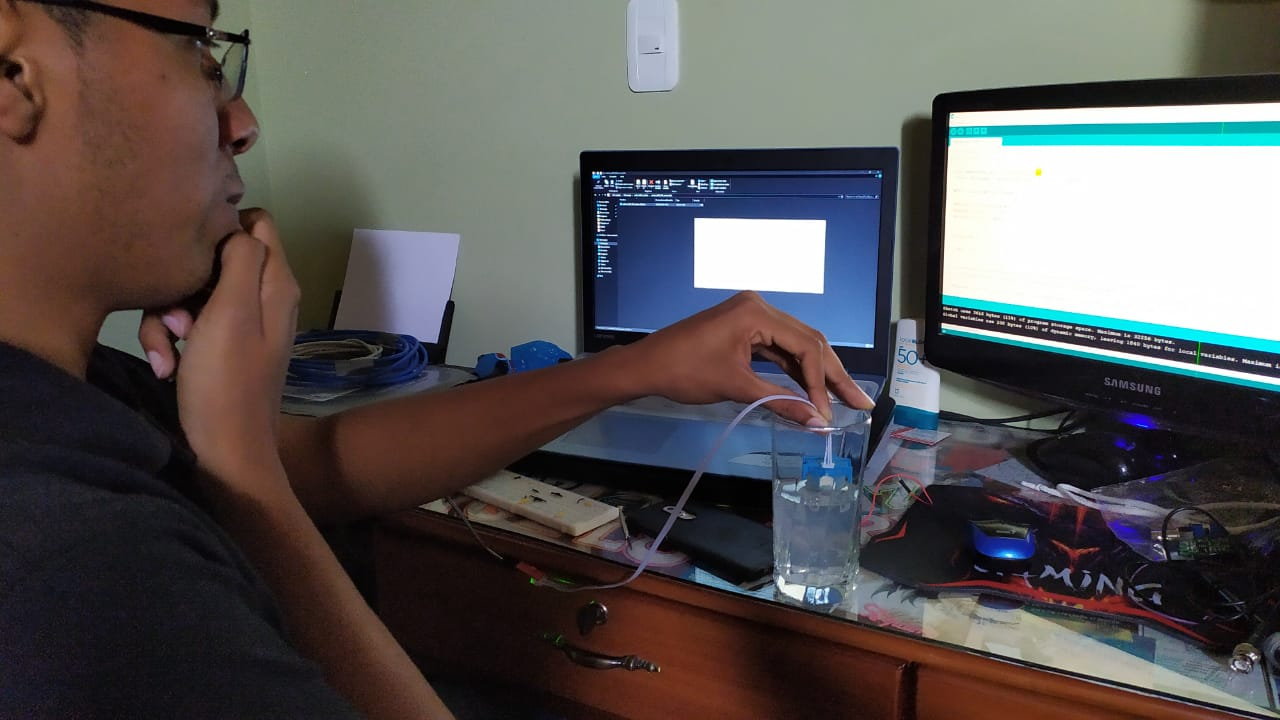
\includegraphics[scale=0.15]{anexo3}
\end{figure}
\begin{figure}[H]
\centering
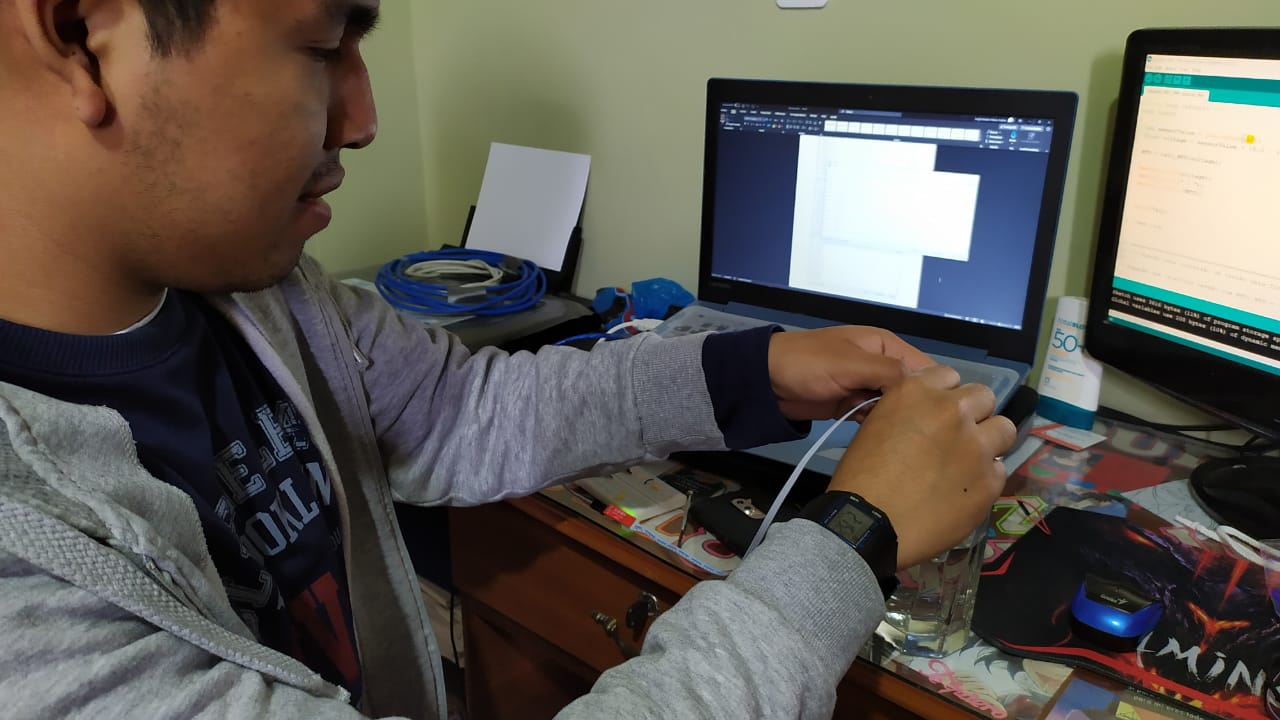
\includegraphics[scale=0.15]{anexo4}
\end{figure}
\begin{figure}[H]
\centering
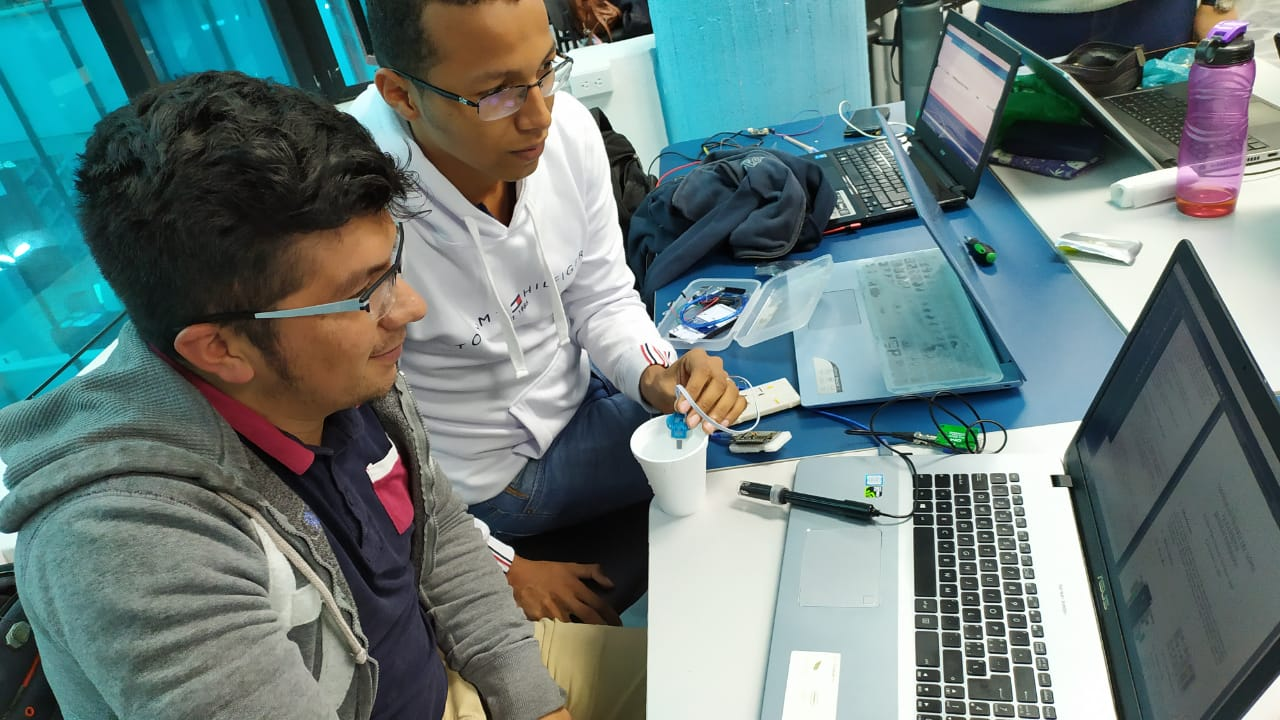
\includegraphics[scale=0.15]{anexo2}
\end{figure}
\begin{figure}[H]
\centering
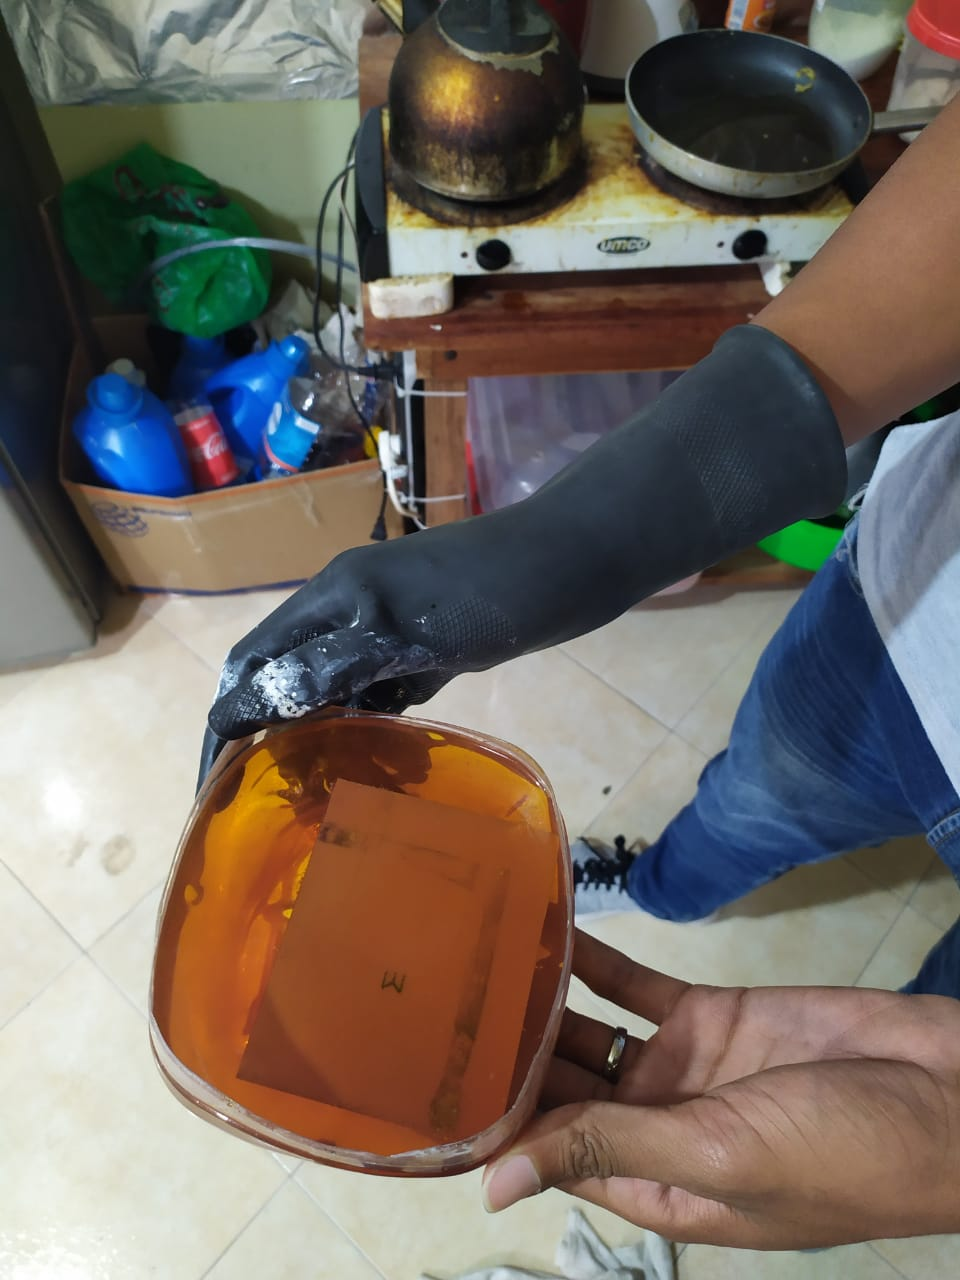
\includegraphics[scale=0.18]{quemar}
\end{figure}
\begin{figure}[H]
\centering
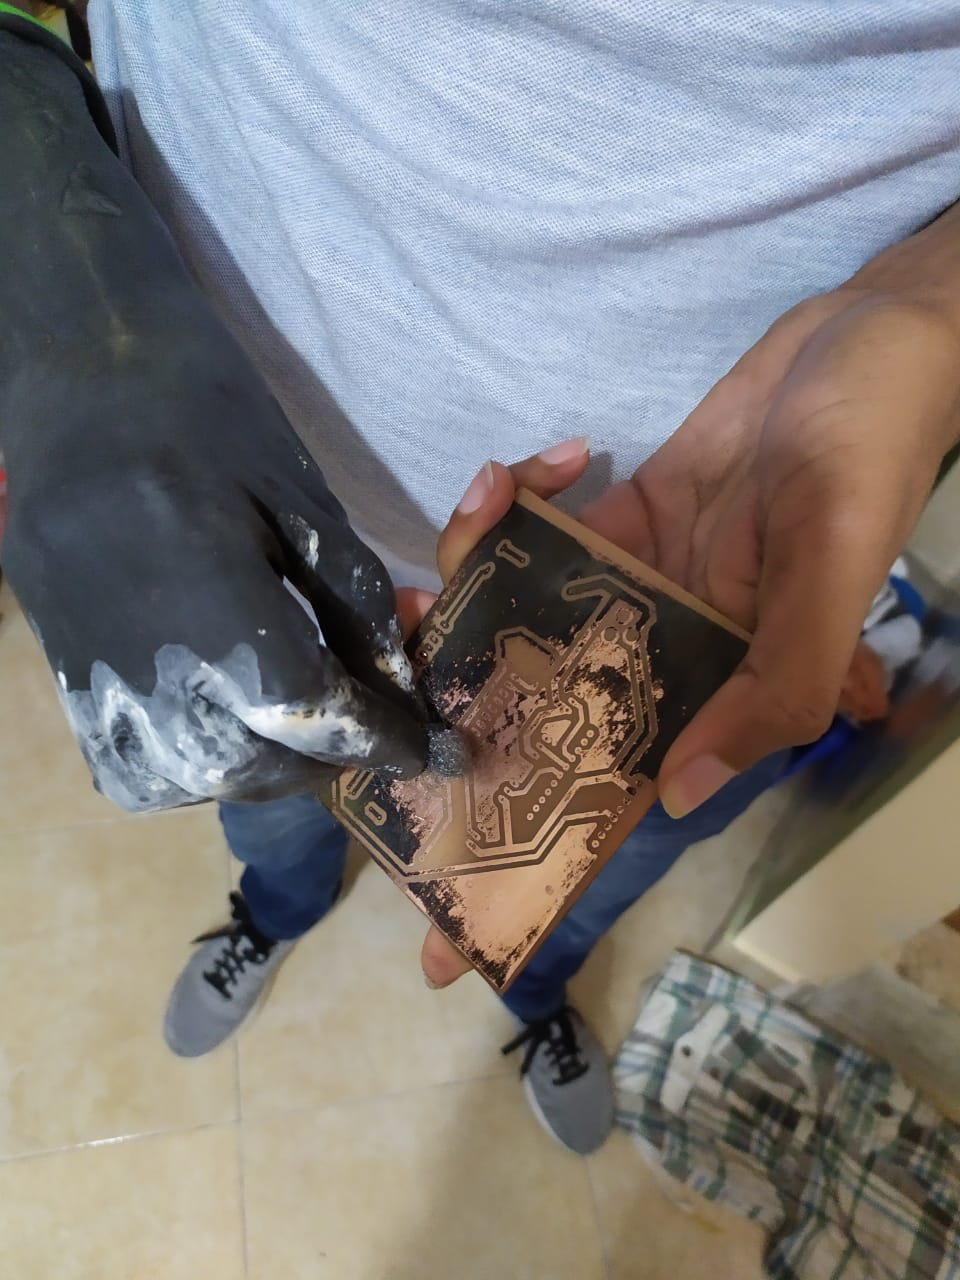
\includegraphics[scale=0.18]{limpiar}
\end{figure}
\begin{figure}[H]
\centering
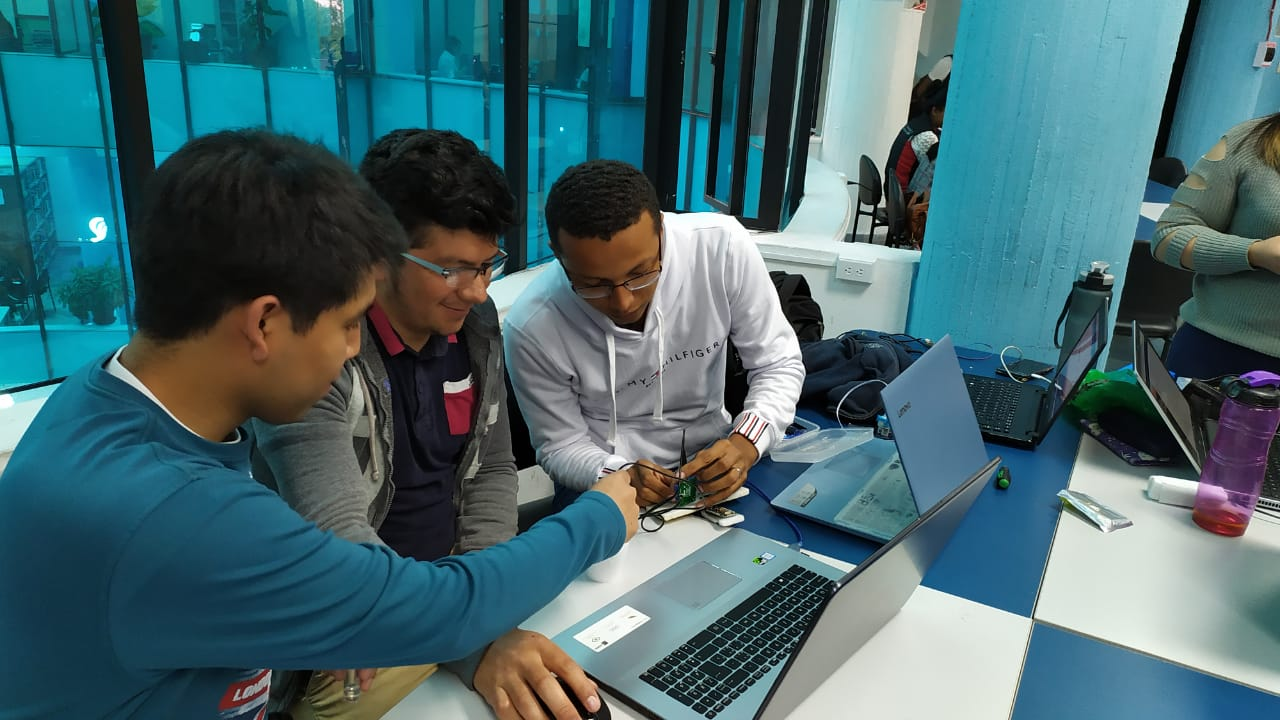
\includegraphics[scale=0.15]{anexo1}
\end{figure}
\begin{figure}[H]
\centering
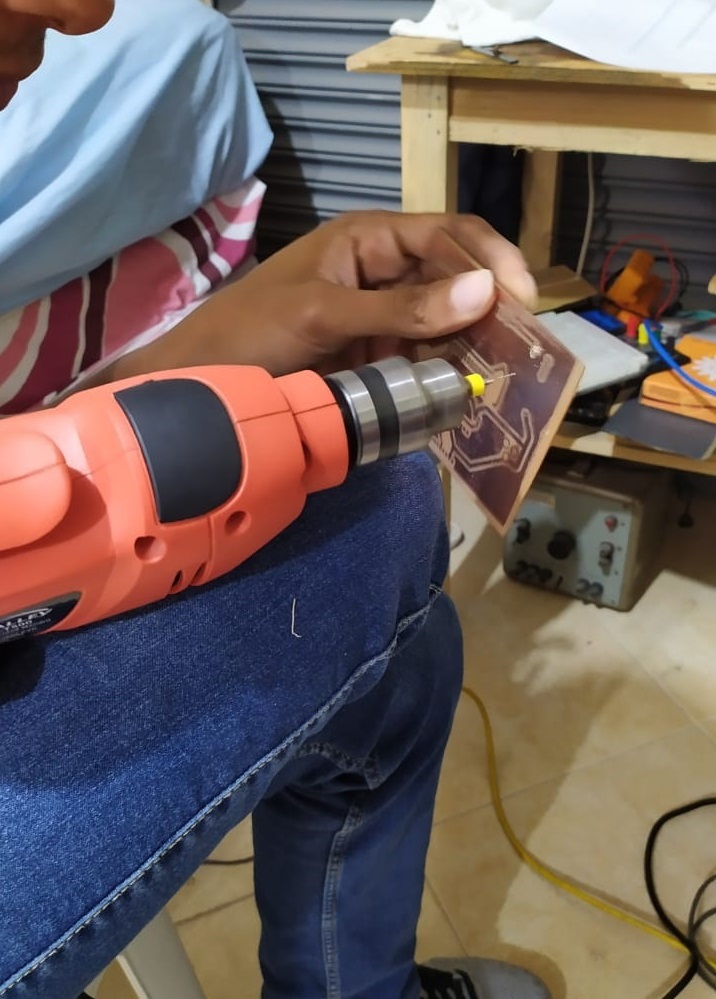
\includegraphics[scale=0.31]{perforar}
\end{figure}
\begin{figure}[H]
\centering
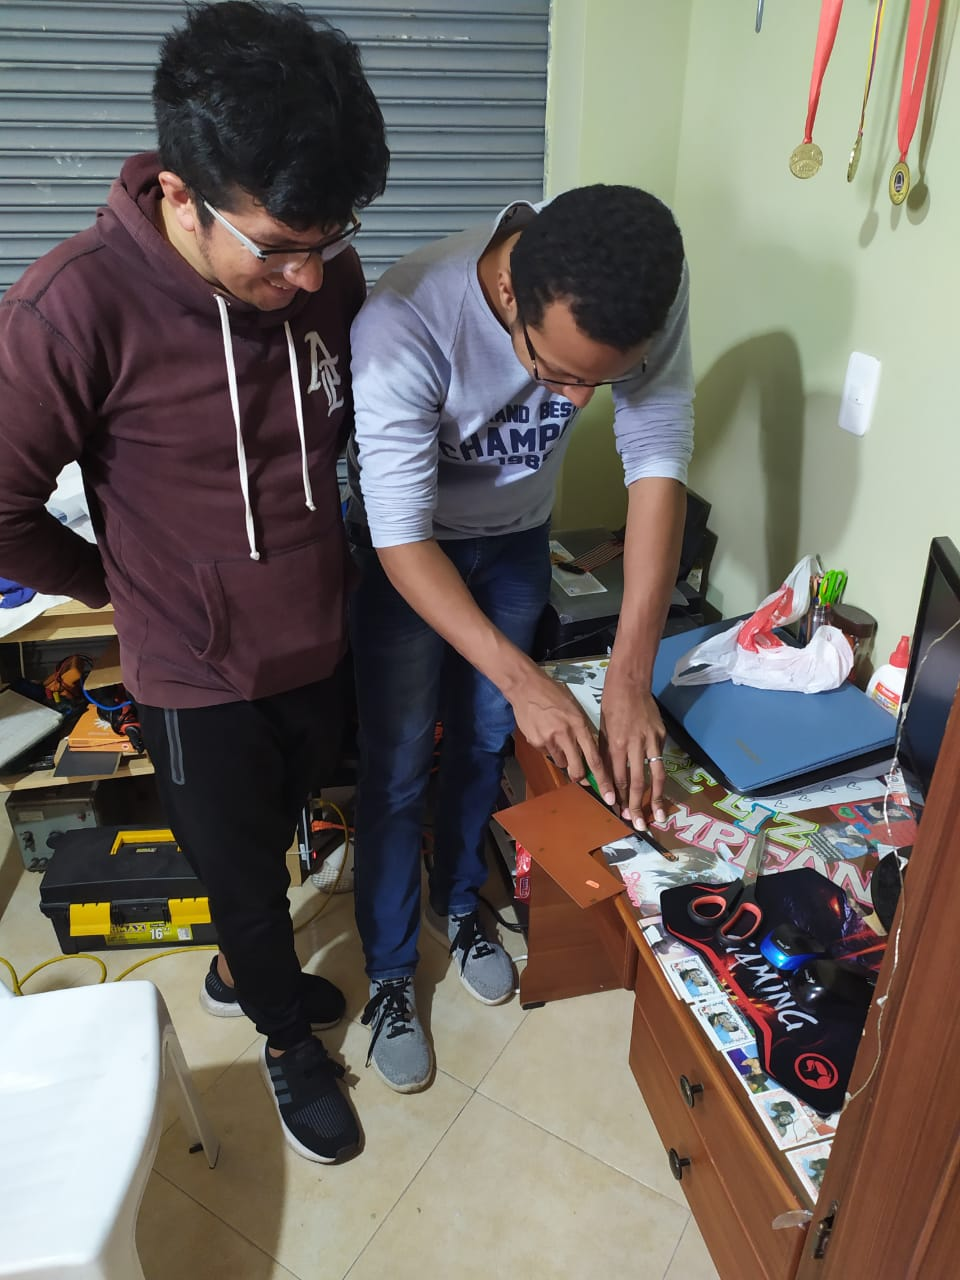
\includegraphics[scale=0.18]{gg}
\end{figure}
\end{multicols}


\bibliographystyle{ieeetran}%estilo referencia
\bibliography{Referencias}%archivo.bib
\end{document}